\section{Validation with $\xi_{\pm}$}
\label{sec:validation}

% Requires the booktabs if the memoir class is not being used
\begin{table}
   \centering
   %\topcaption{Table captions are better up top} % requires the topcapt package
    \caption{IA models infused in this work and the respective fiducial values of the model parameters.}
   \begin{tabular}{@{} lcr @{}} % Column formatting, @{} suppresses leading/trailing space
      \hline
      \hline
      %\multicolumn{2}{c}{Item} \\
      model   		& ($A_{\rm IA}, \: b_{\rm TA}, \: A_2)$ \\
      \hline
      NLA     		& ($\pm$1, 0, 0) &  \\
      \hline
      \multirow{2}{*}{extended-NLA }  	&   ($\pm$1, 1, 0)   \\
                                        &  (1, 2, 0)   \\
      \hline
      TT 			&  {(0, 0, $\pm$1)} &  \\
      \hline
      \multirow{2}{*}{extended-TT} 	    &  (0, 1 ,$\pm$1)   \\
                                        &  (0, 2, 1)   \\
      \hline
      TATT- fiducial	&  (1, 1, 1)  \\
      \hline
      \hline
   \end{tabular}
   \label{table:IAmodels}
\end{table}



%------------------------------
\subsection{NLA model}
\label{subsubsec:sigma_G}

See Fig. \ref{fig:xi_NLA}

%---------------
\begin{figure*}
%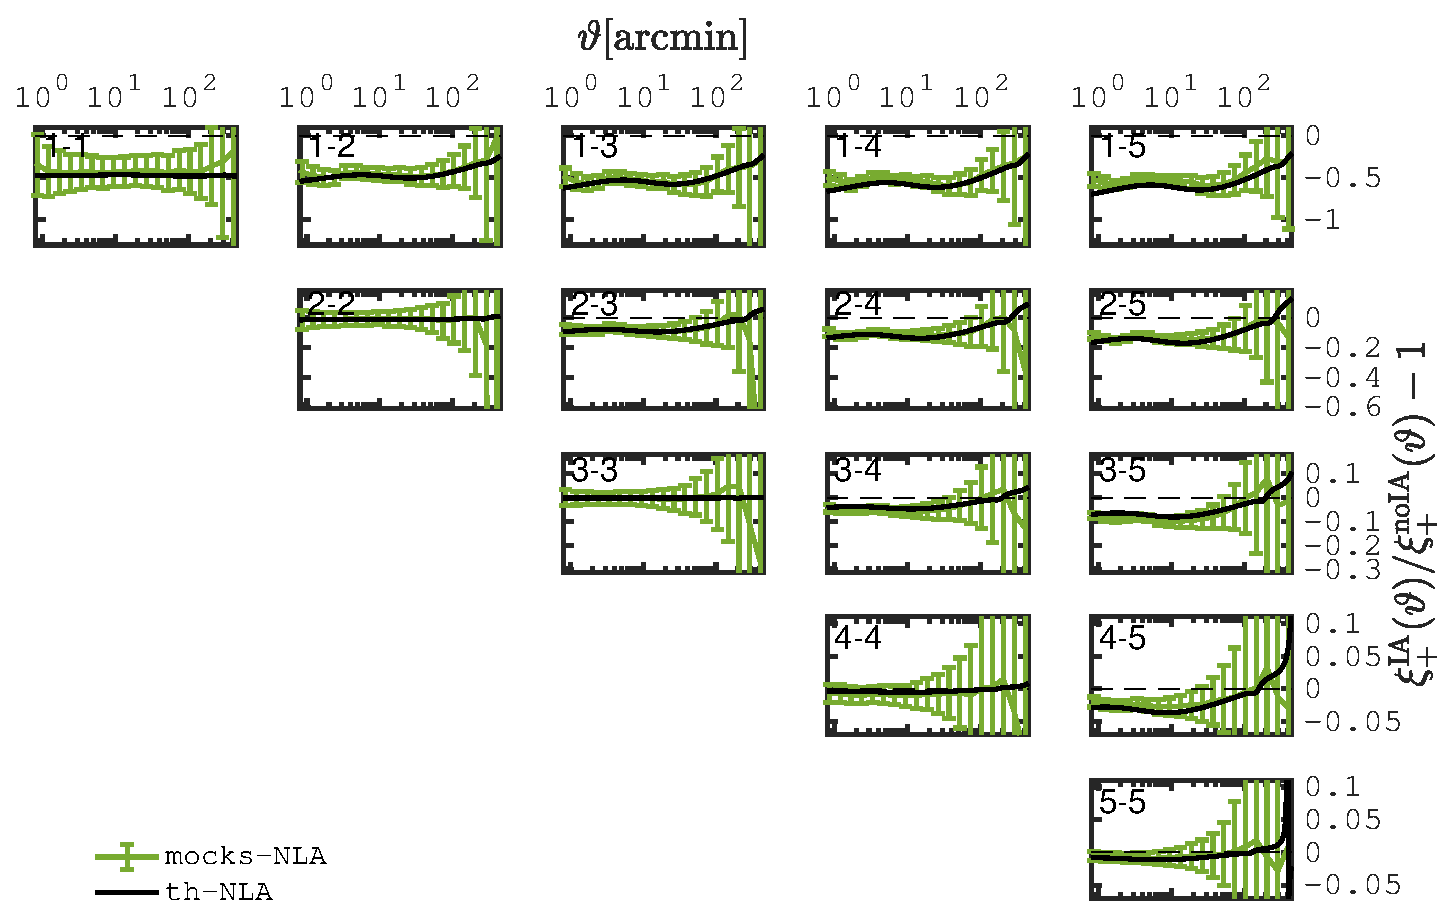
\includegraphics[width=\columnwidth]{graphs/frac_xip_IA1_skysim}
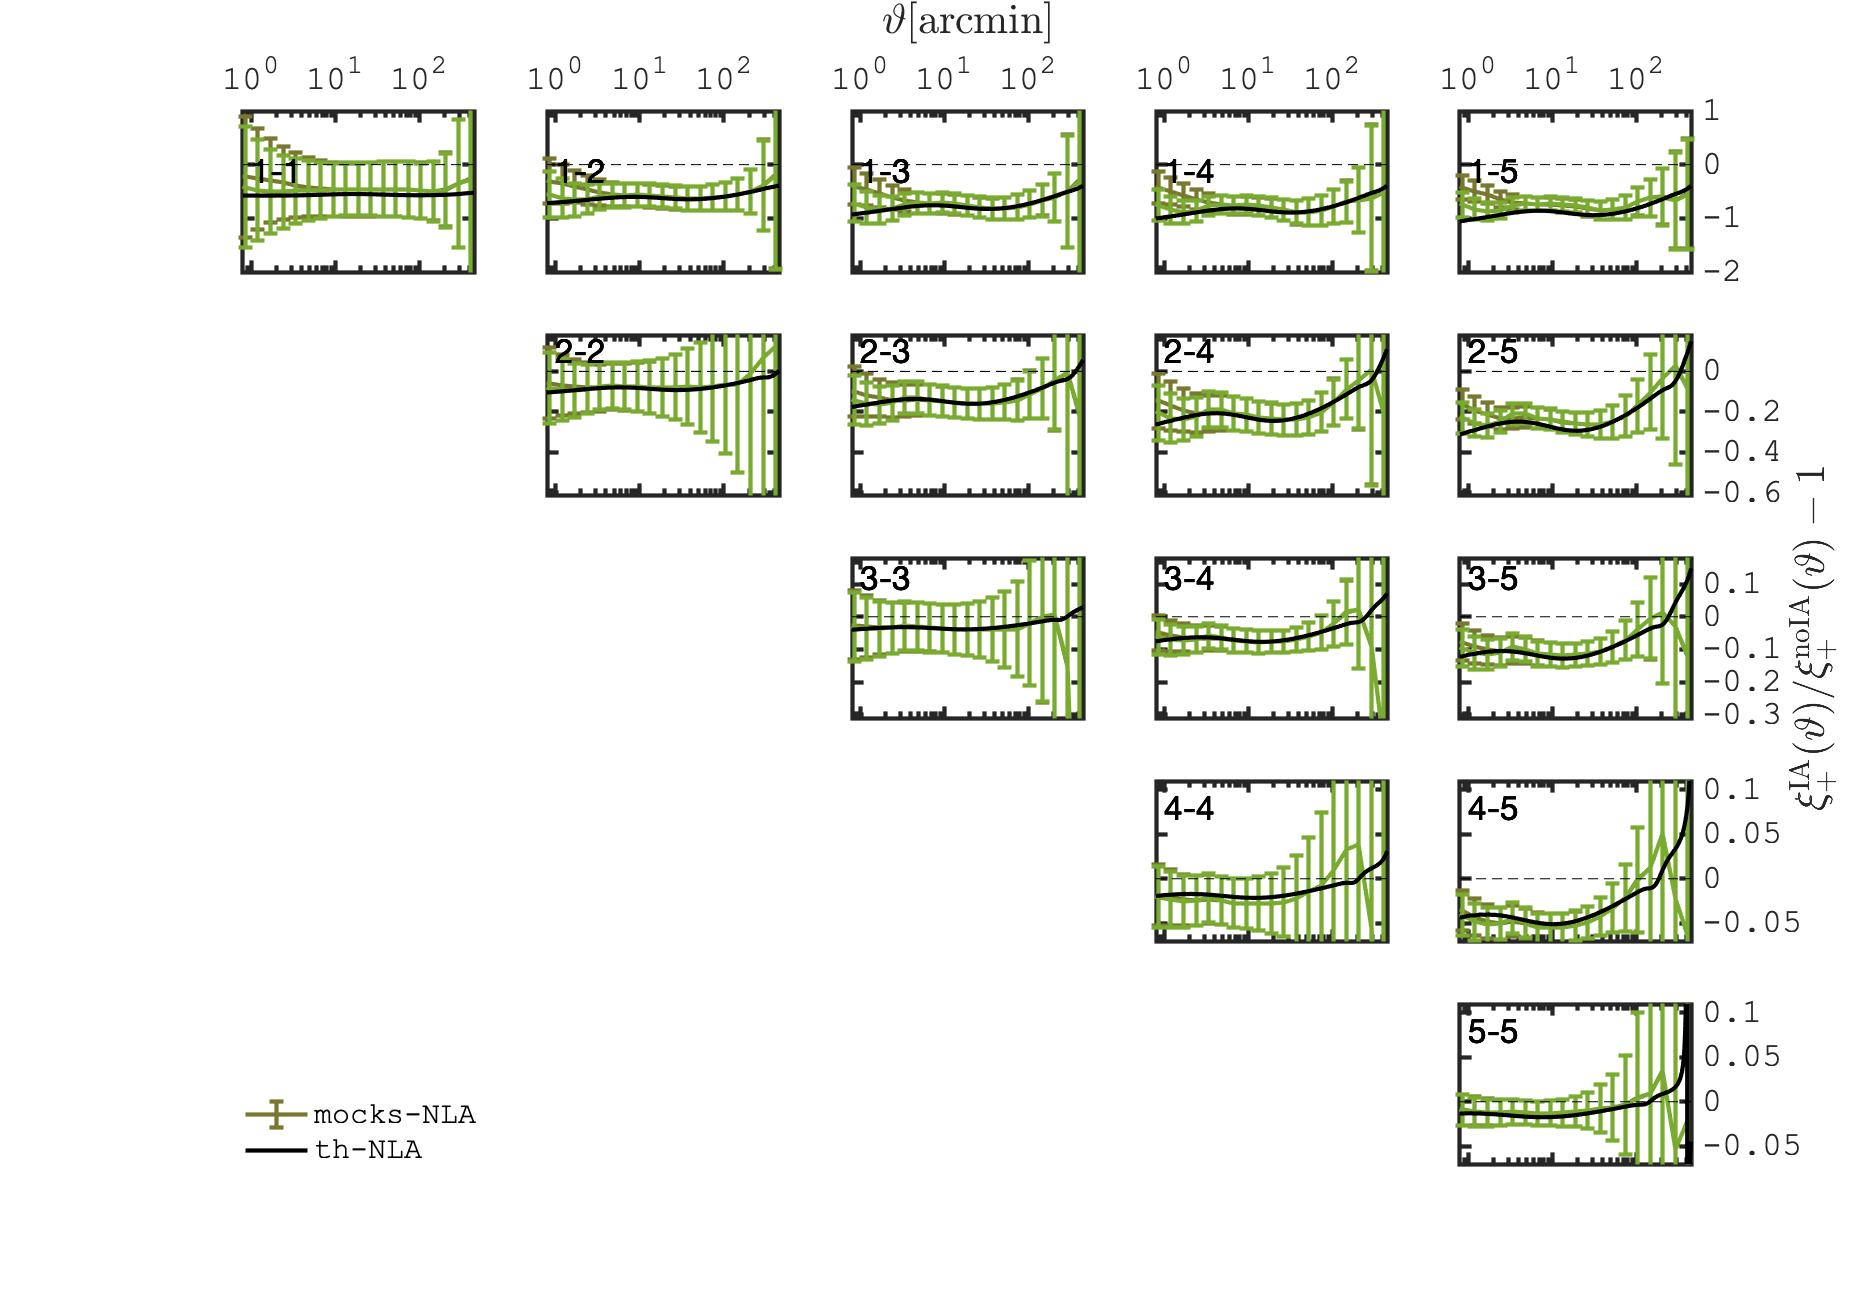
\includegraphics[width=\columnwidth]{graphs/frac_xip_IA1_skysim_NLA_srd.jpg}
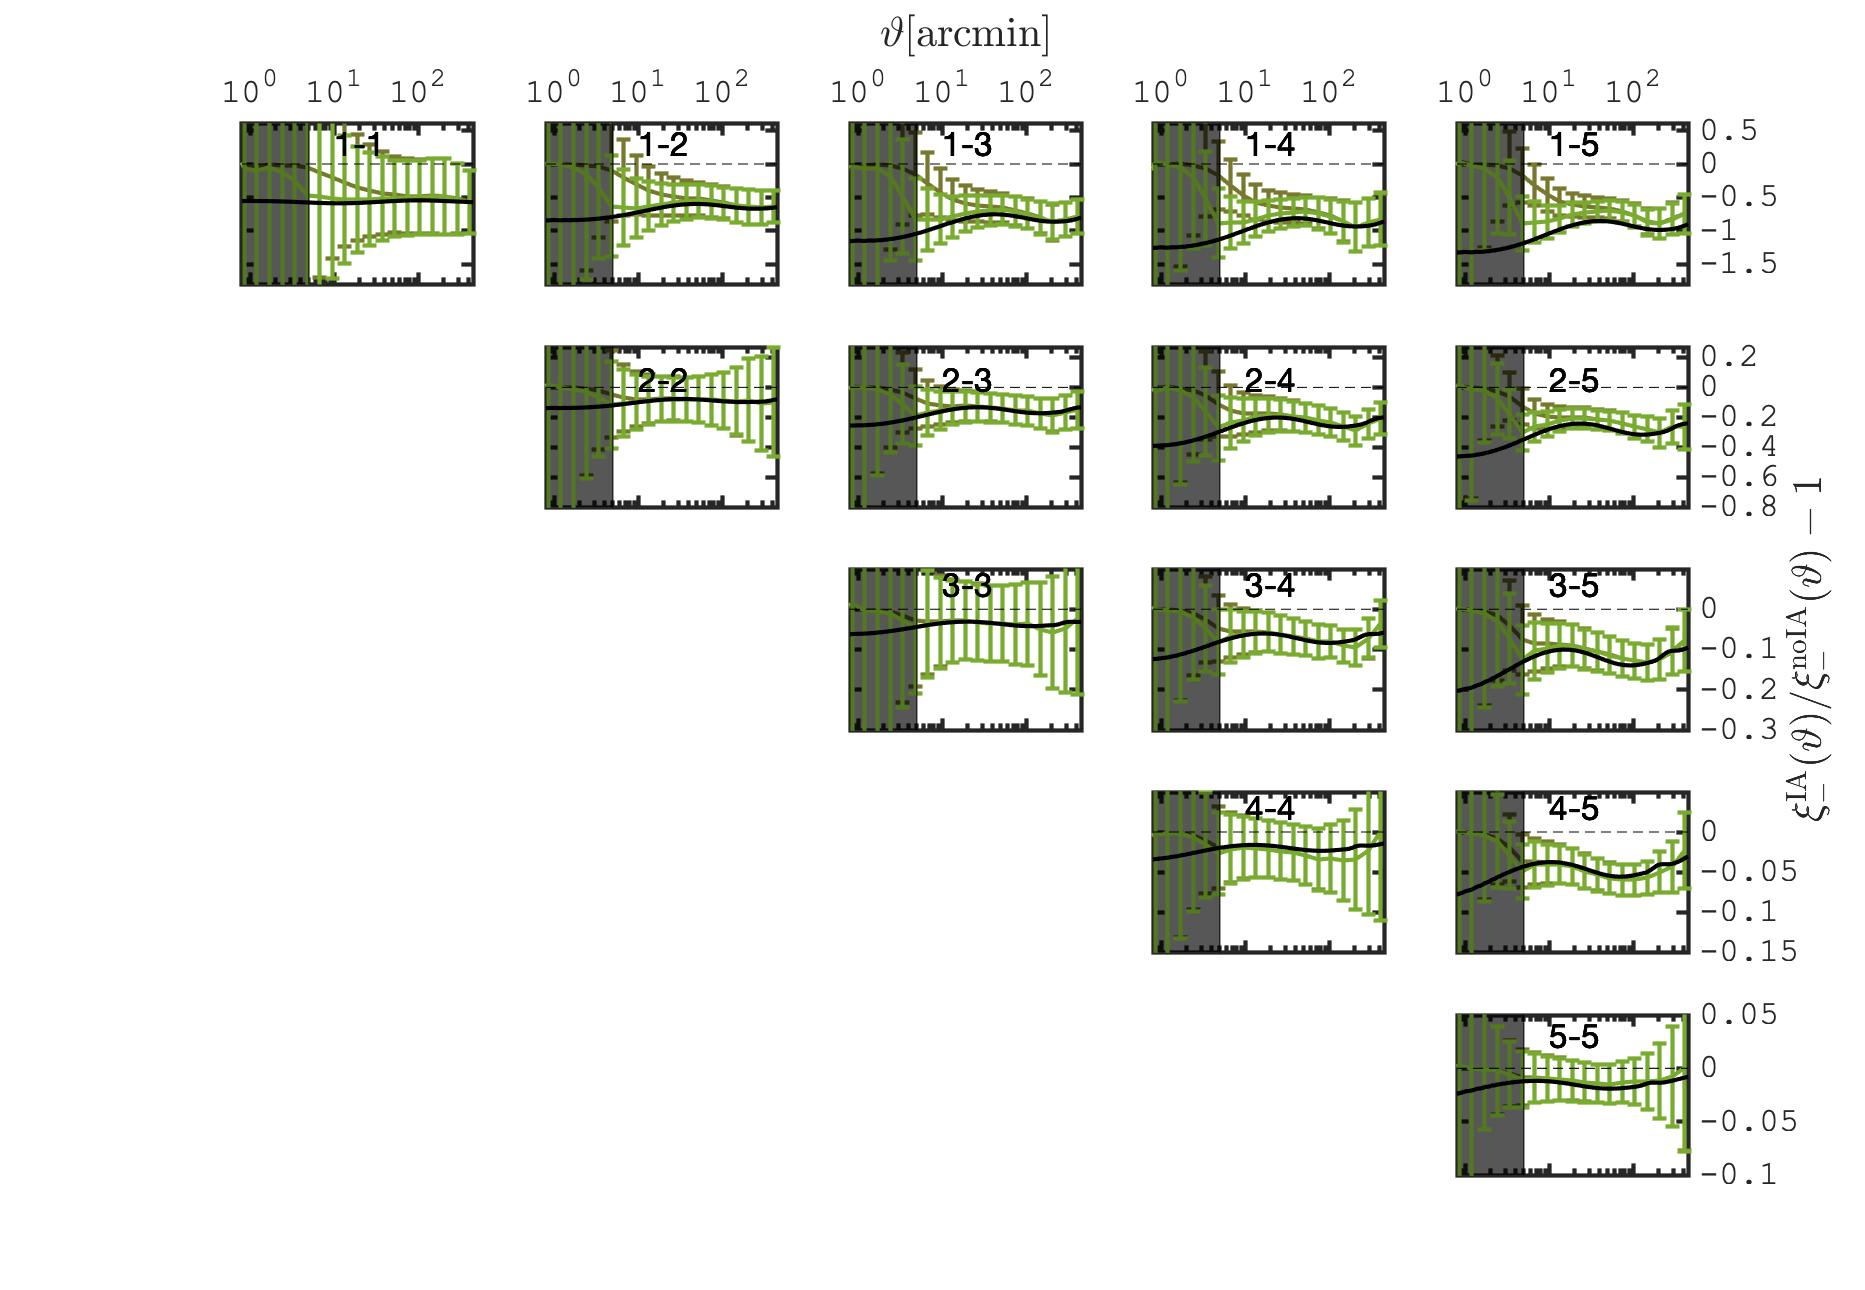
\includegraphics[width=\columnwidth]{graphs/frac_xim_IA1_skysim_NLA_srd.jpg}
\caption{Ratio between the shear correlation functions with and without IA, assuming the NLA model with $A_{\rm IA}=1.0$ both in the simulations and theory. Measurements shown in green and brown correspond to smoothing scales of 0.1 and 0.5 $h^{-1}$Mpc in the tidal field. There is no shape noise in the simulations, but it is included in the error bars.}
\label{fig:xi_NLA}
\end{figure*}
%---------------

%------------------------------
\subsection{Extended-NLA model}
\label{subsec:deltaNLA}

See Fig. \ref{fig:xi_deltaNLA}.

\begin{figure*}
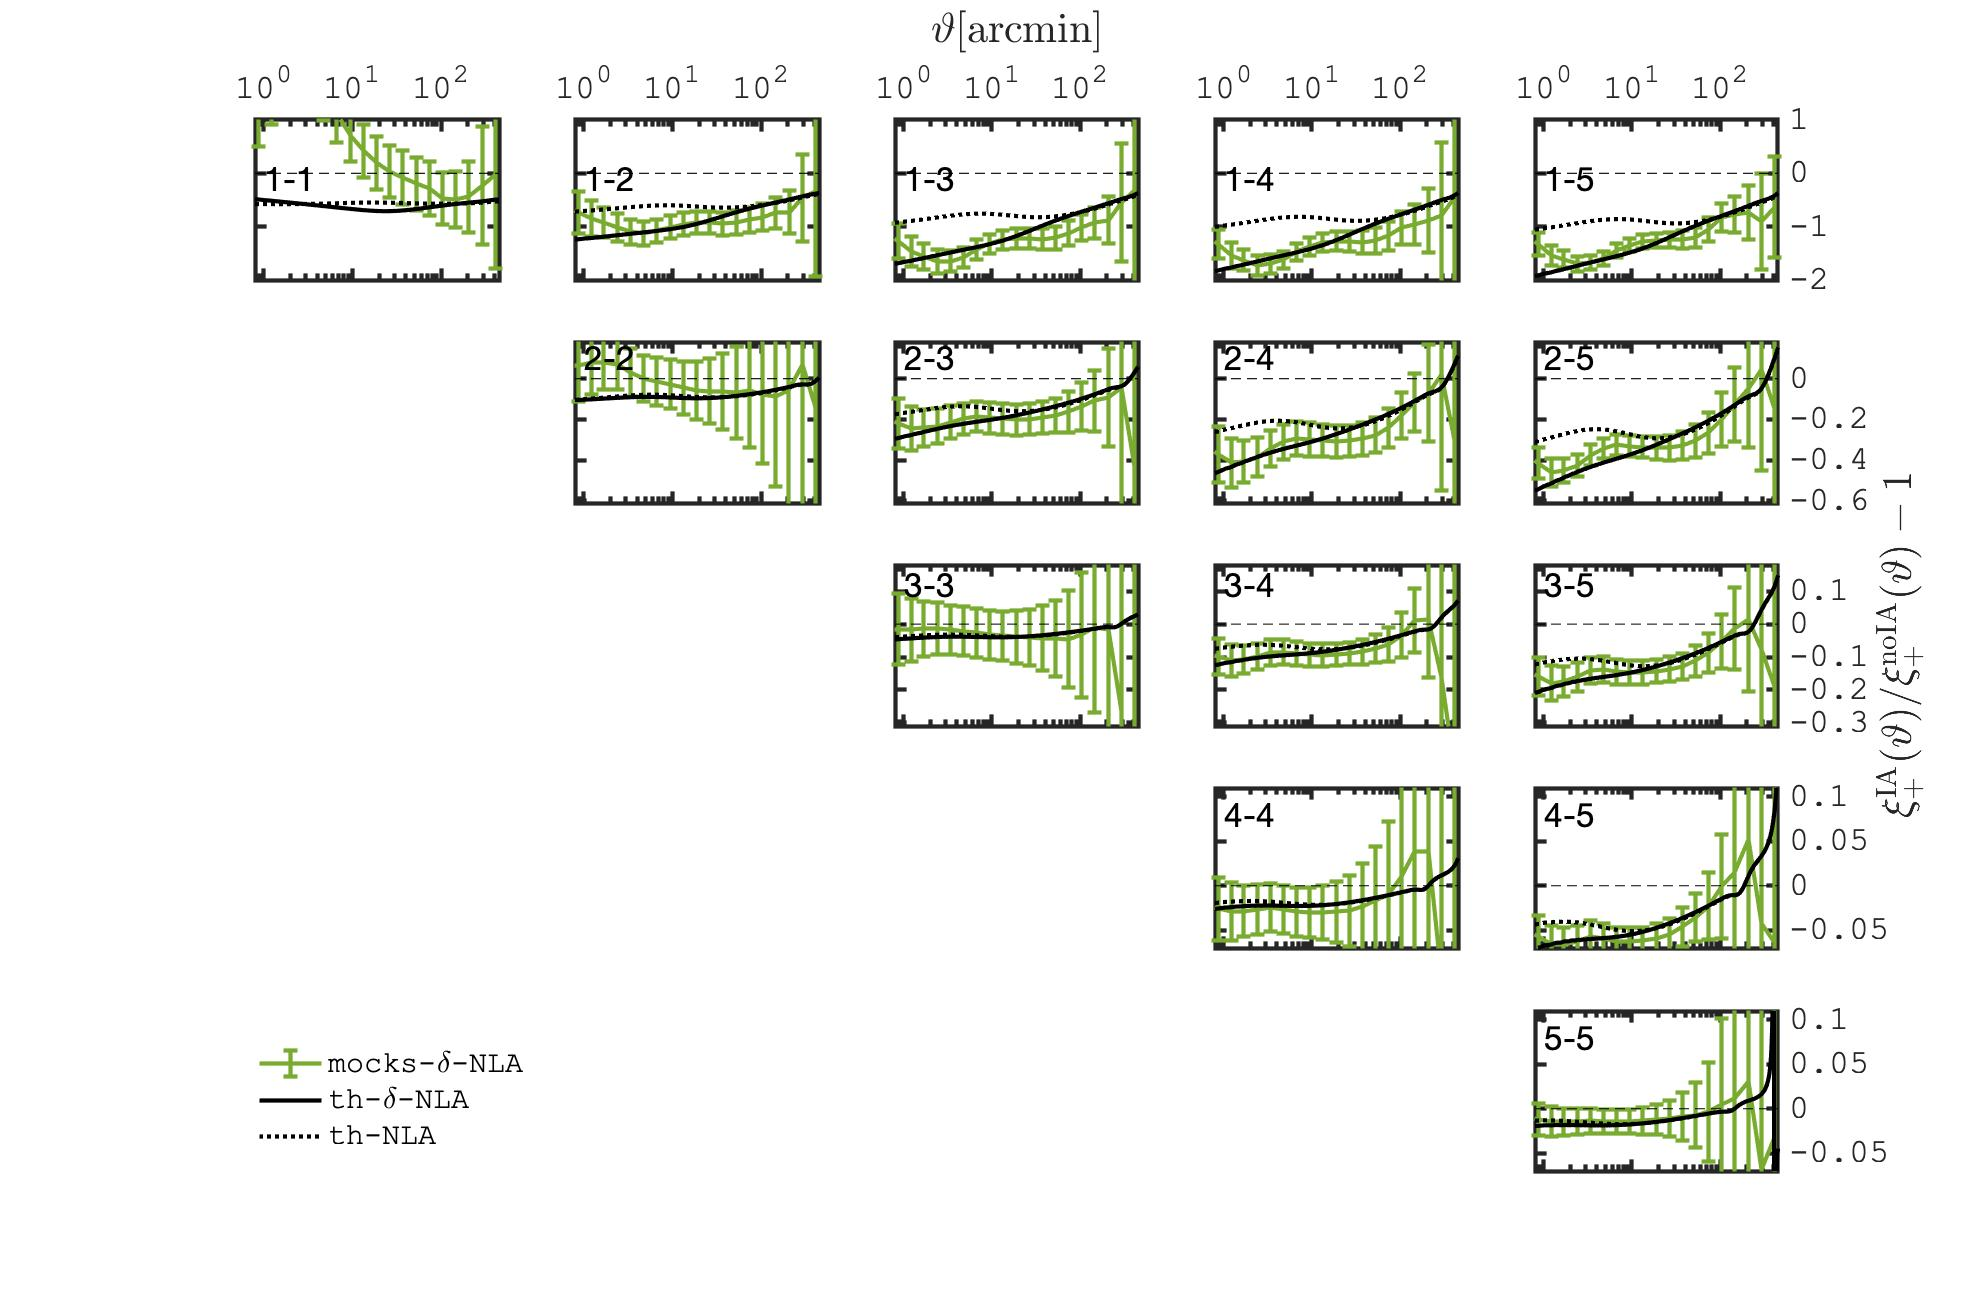
\includegraphics[width=\columnwidth]{graphs/frac_xip_IA1_skysim_deltaNLA_srd}
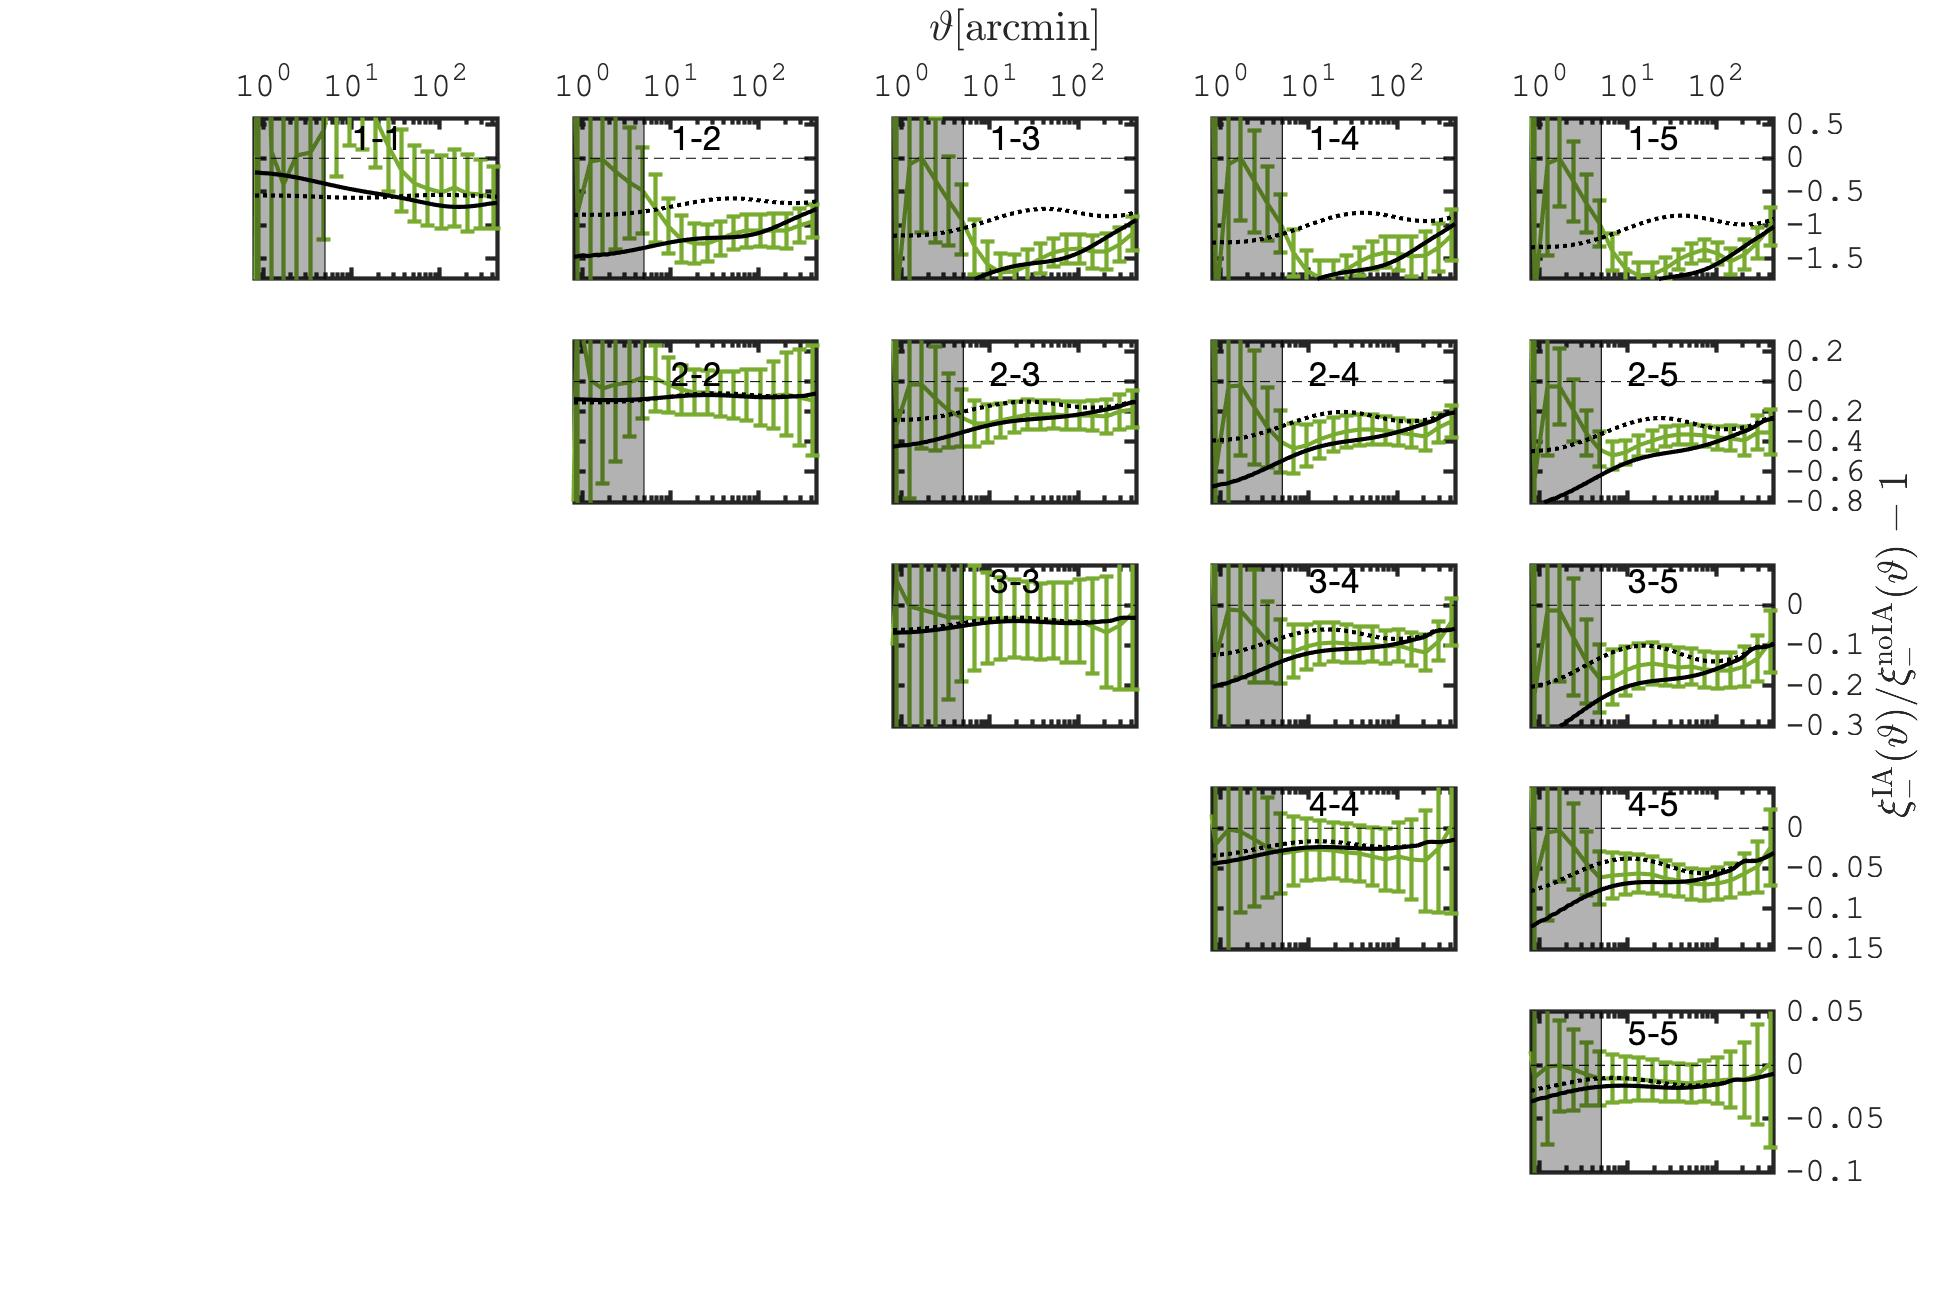
\includegraphics[width=\columnwidth]{graphs/frac_xim_IA1_skysim_deltaNLA_srd}
\caption{Same as Fig. \ref{fig:xi_NLA}, but for the $\delta$-NLA model with $A_{\rm IA}=1.0$ and $b_{\rm TA}=1.0$, and only for smoothing of 0.5$h^{-1}$Mpc. The dashed black lines show the NLA predictions to better highlight the differences.  }
\label{fig:xi_deltaNLA}
\end{figure*}

\begin{figure}
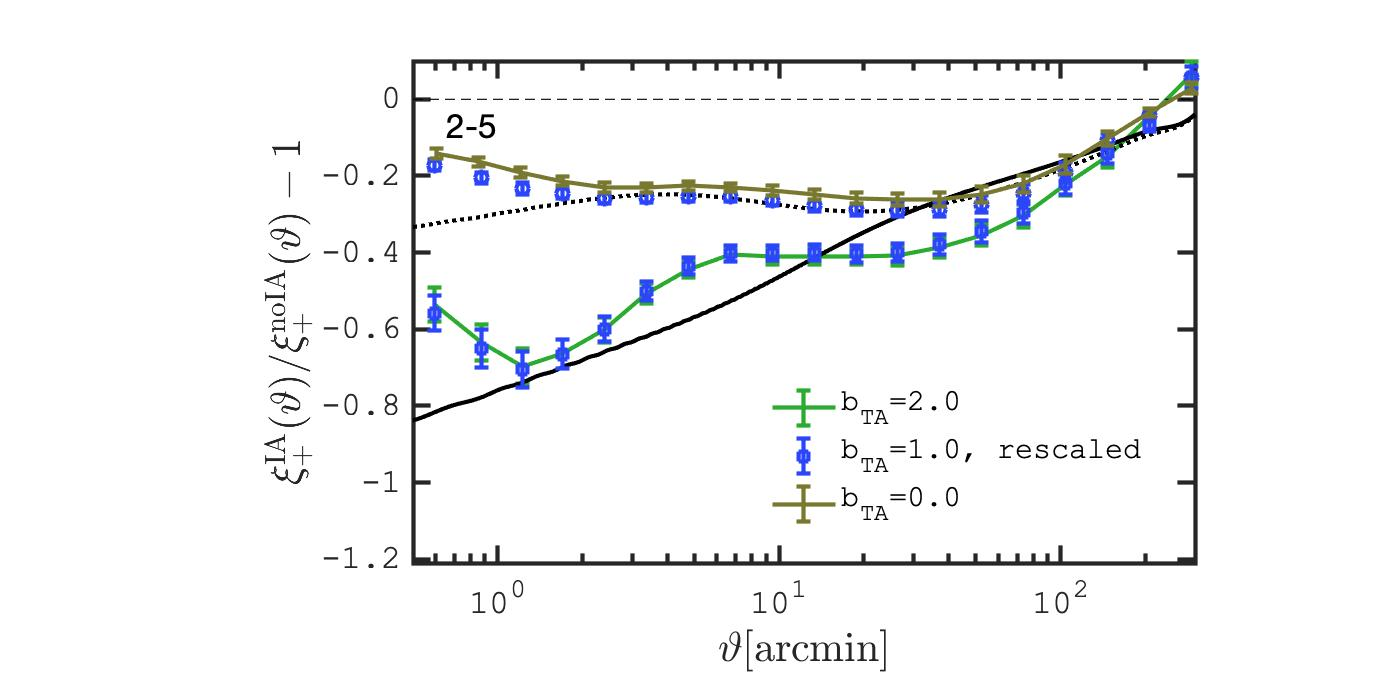
\includegraphics[width=\columnwidth]{graphs/frac_xip_bta1_rescaled}
\caption{Ratio between the shear correlation functions with and without IA in tomographic bin combination 2-5.
The brown and green symbols show measurements from simulations constructed with $b_{\rm TA}$ = 0.0 and 2.0 respectively,  the black solid and dotted lines shown their predictions, while the blue symbols are obtained by rescaling $b_{\rm TA}$ = 1.0 simulations using Eq. \ref{eq:bta_rescale}.  }
\label{fig:xi_deltaNLA_rescaled}
\end{figure}


We verified that it works equally well for $b_{\rm TA}$ = 1.0 and 2.0.

%------------------------------

Using this, we $b_{\rm TA}$-rescale our $b_{\rm TA}=1.0$ mock to $b_{\rm TA}=2.0$ and to $0.0$ mocks. Results are shown in Fig. \ref{fig:xi_deltaNLA_rescaled} for one of the tomographic bin. 
It works reasonably well, but lower redshift are less accurate due to the increased  shot noise (not shown), hence we do not recommend using this.

%------------------------------
\subsection{TT model}
\label{subsec:TT}

See Fig. \ref{fig:xi_TT}

\begin{figure*}
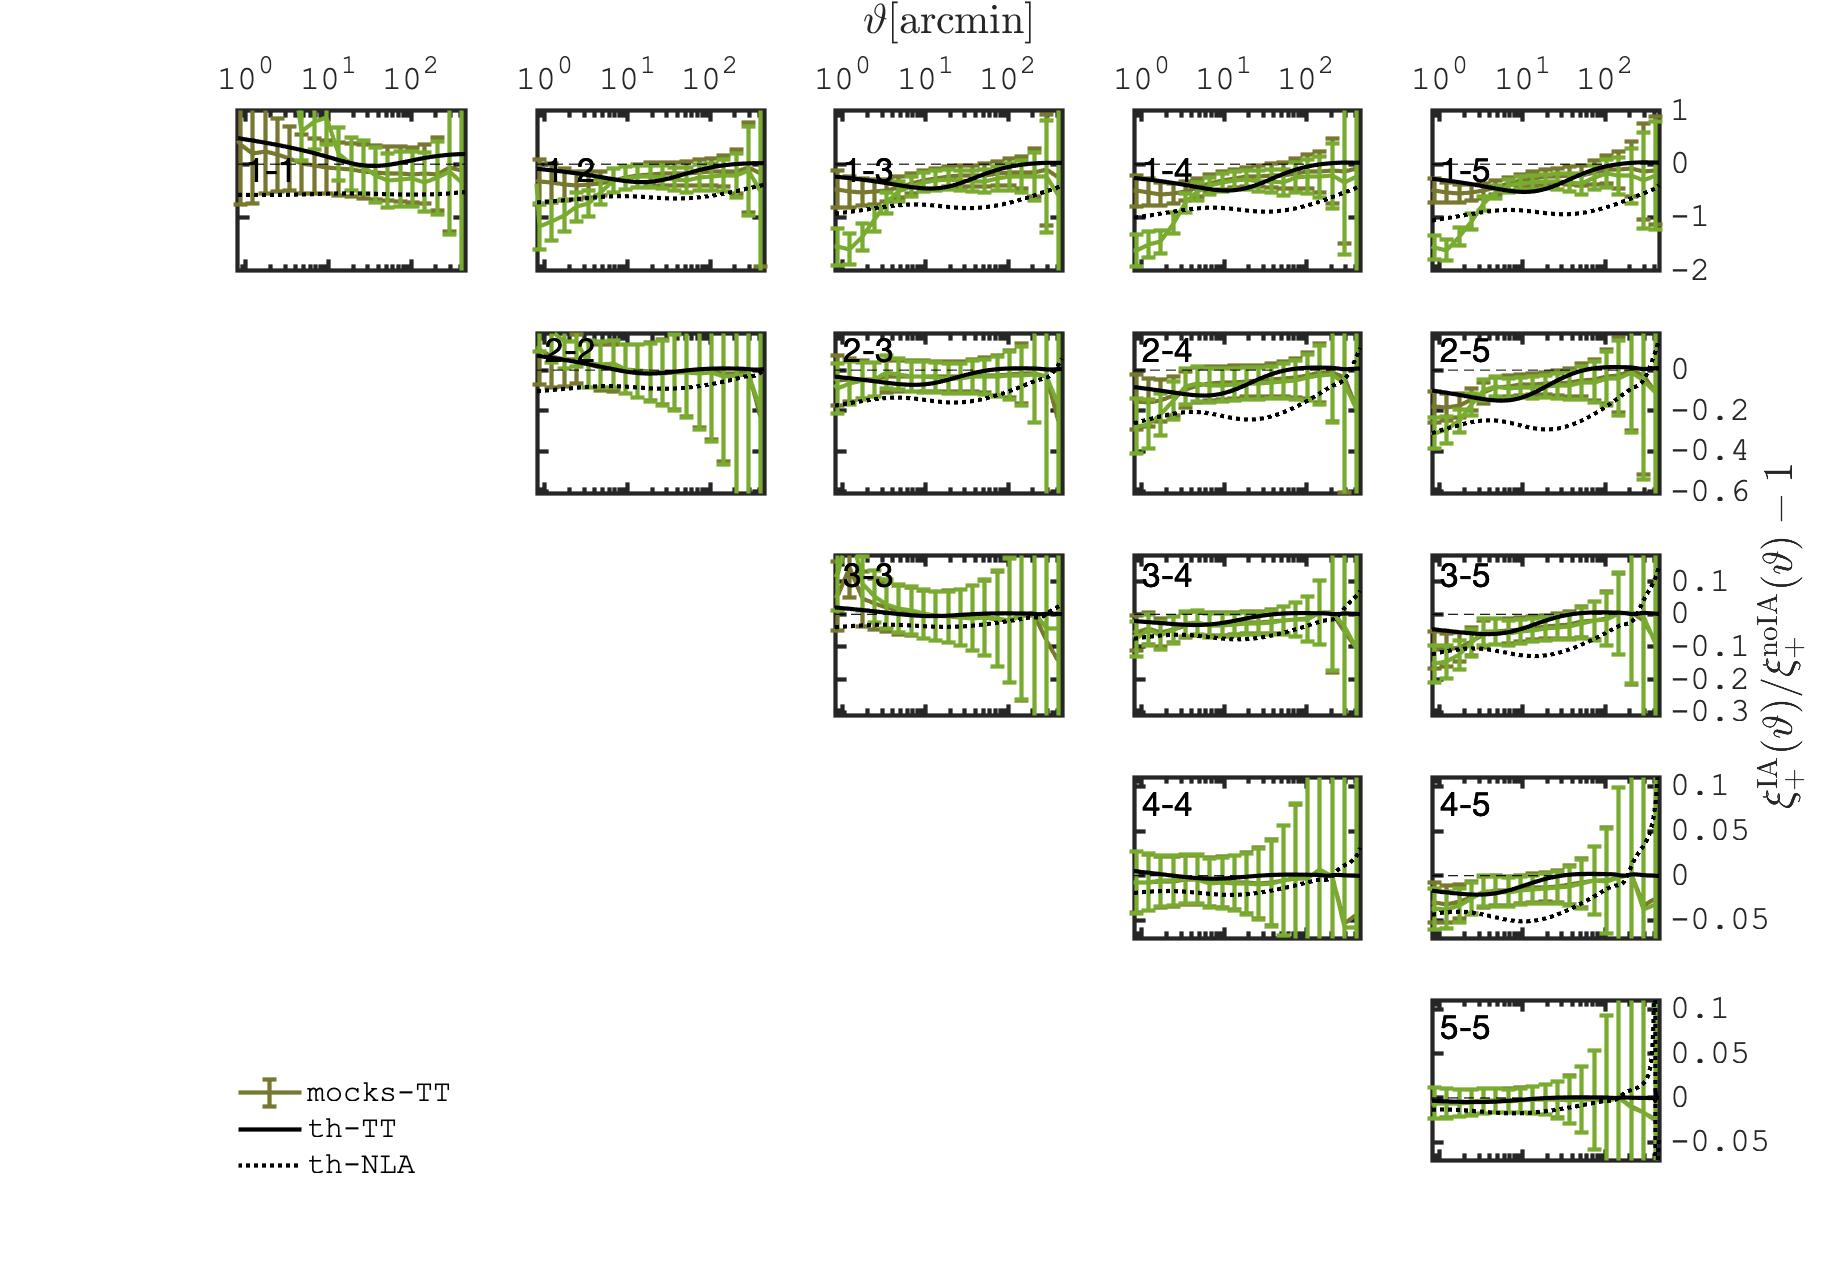
\includegraphics[width=\columnwidth]{graphs/frac_xip_IA1_skysim_TT_srd.jpg}
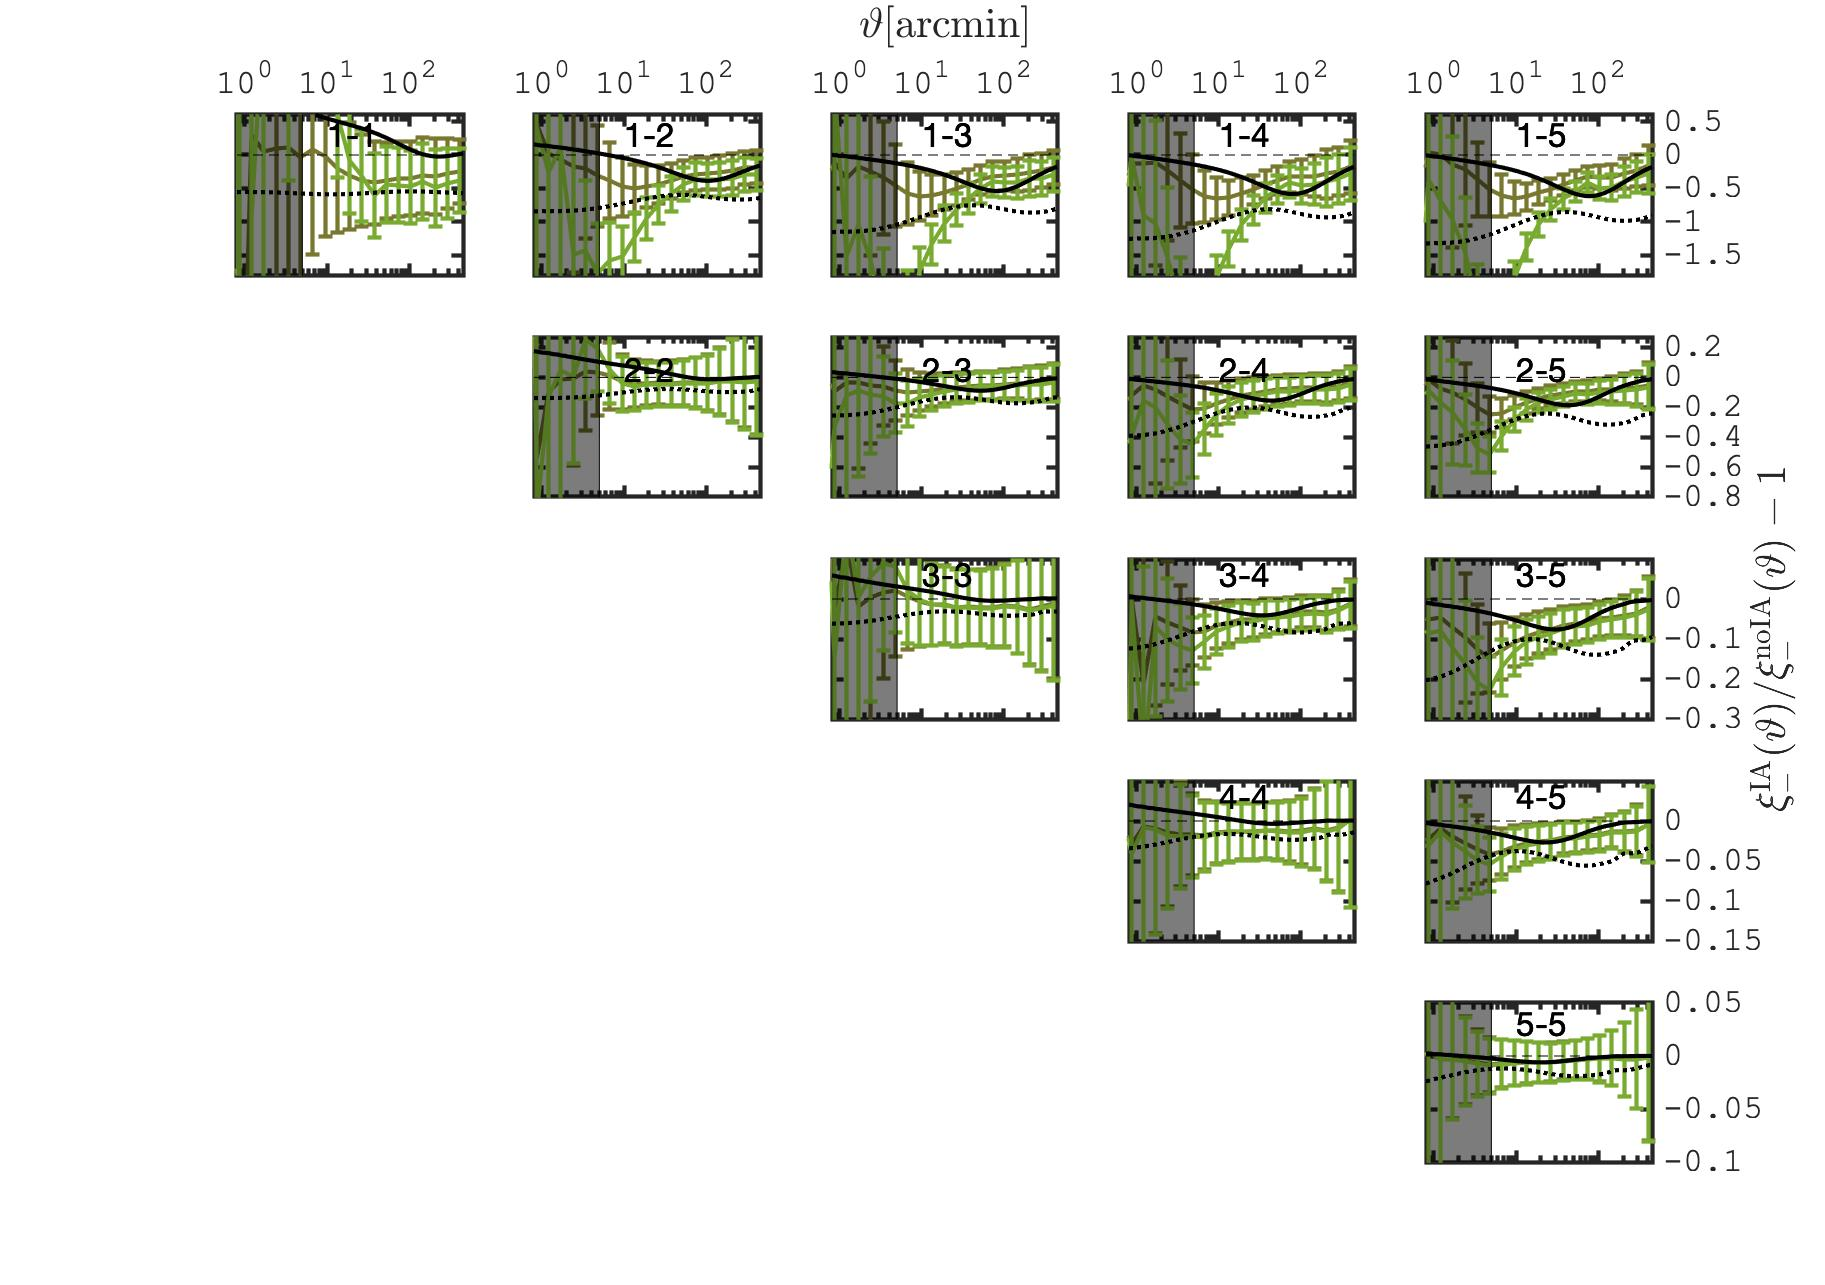
\includegraphics[width=\columnwidth]{graphs/frac_xim_IA1_skysim_TT_srd.jpg}
\caption{Same as Fig. \ref{fig:xi_NLA}, but for the TT model with $A_2=1.0$. Brown is smoothing scale of 0.5 arcmin, green is 0.1 arcmin. Here, the dashed black lines show the NLA predictions to better highlight the differences. }
\label{fig:xi_TT}
\end{figure*}

\begin{figure*}
%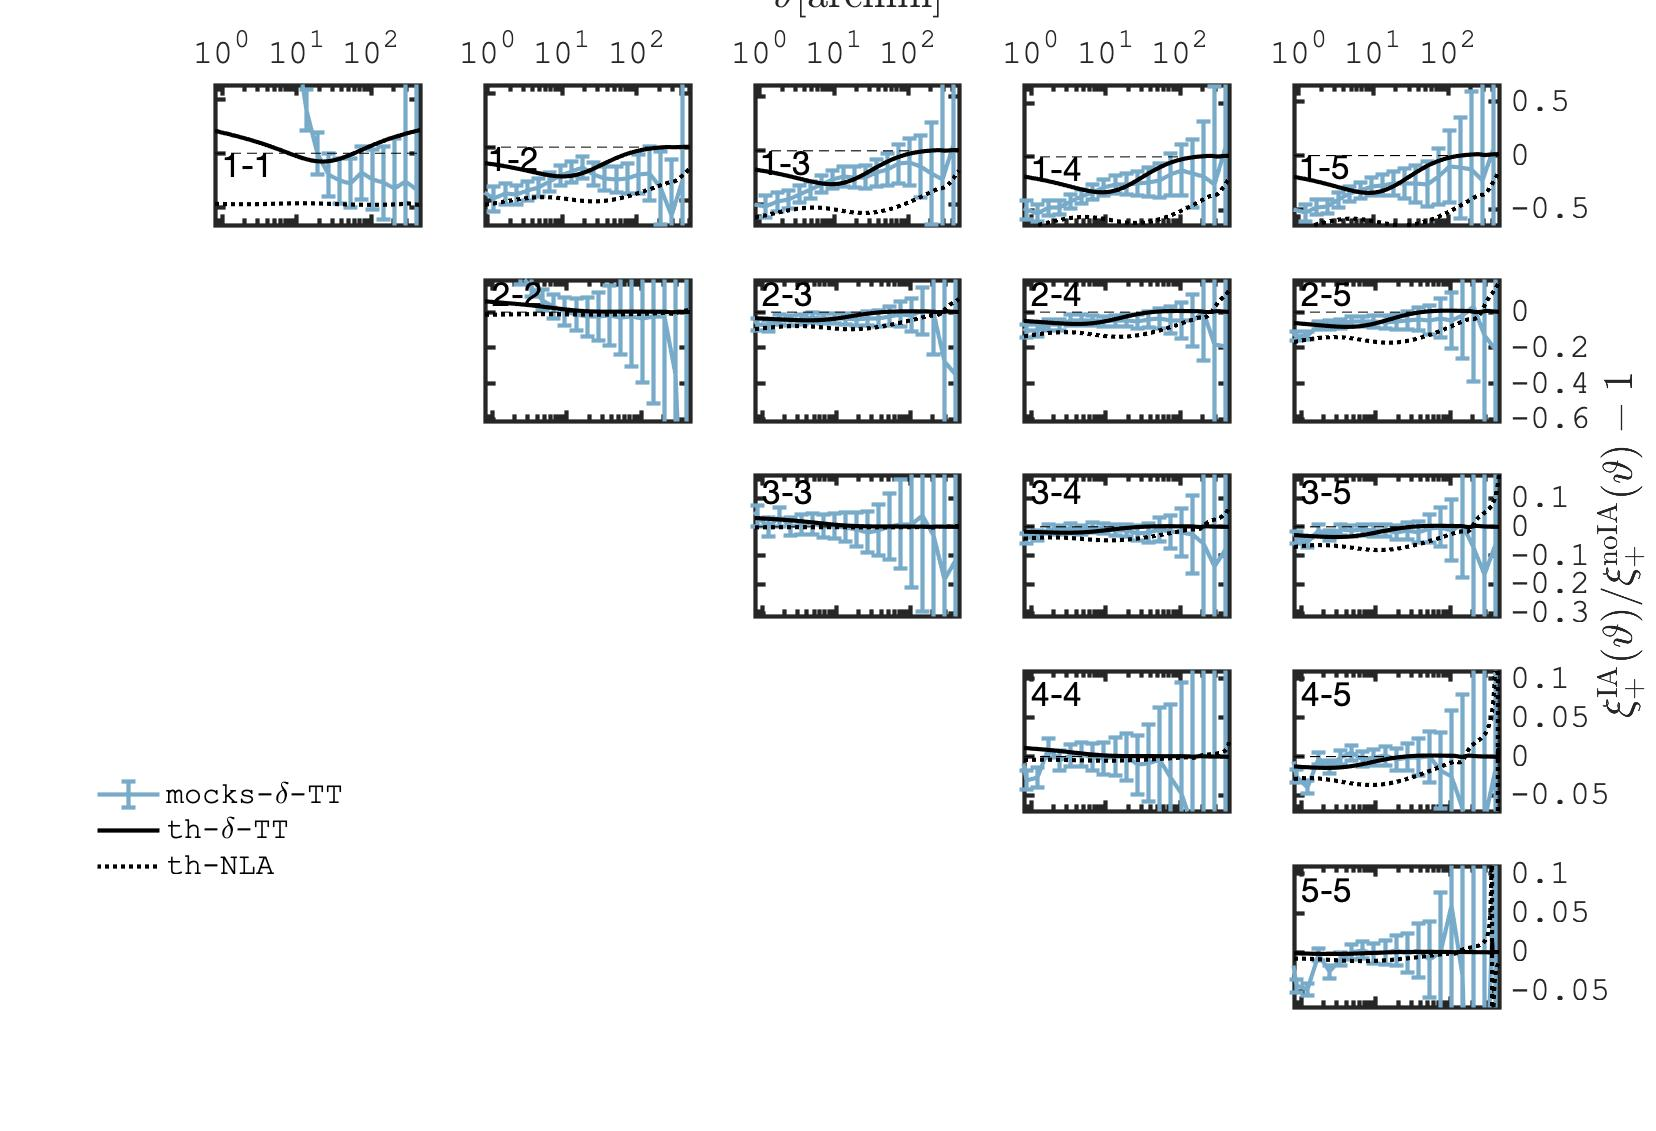
\includegraphics[width=\columnwidth]{graphs/frac_xip_C2_m1_skysim_deltaTT}
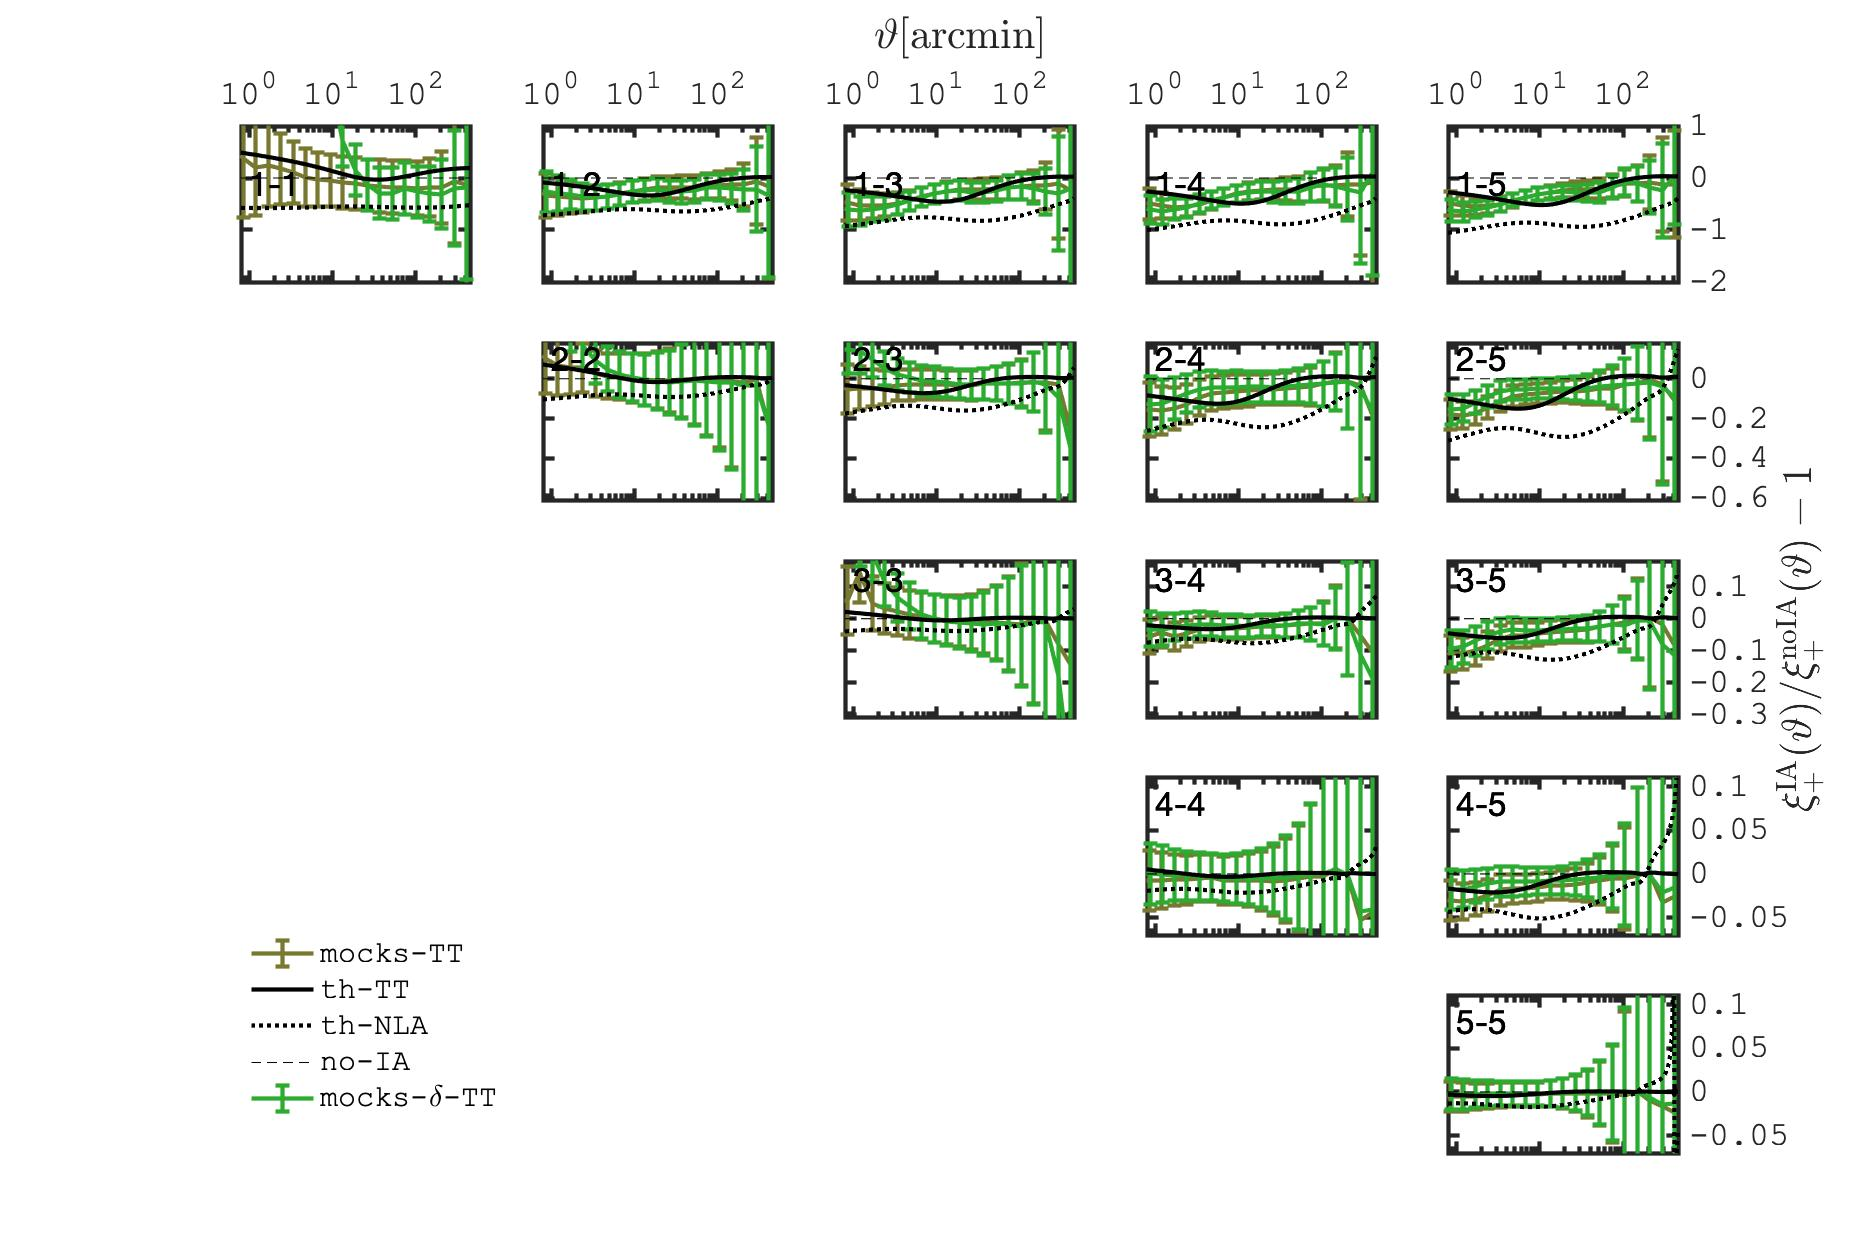
\includegraphics[width=\columnwidth]{graphs/frac_xip_IA1_skysim_deltaTT_srd.jpg}
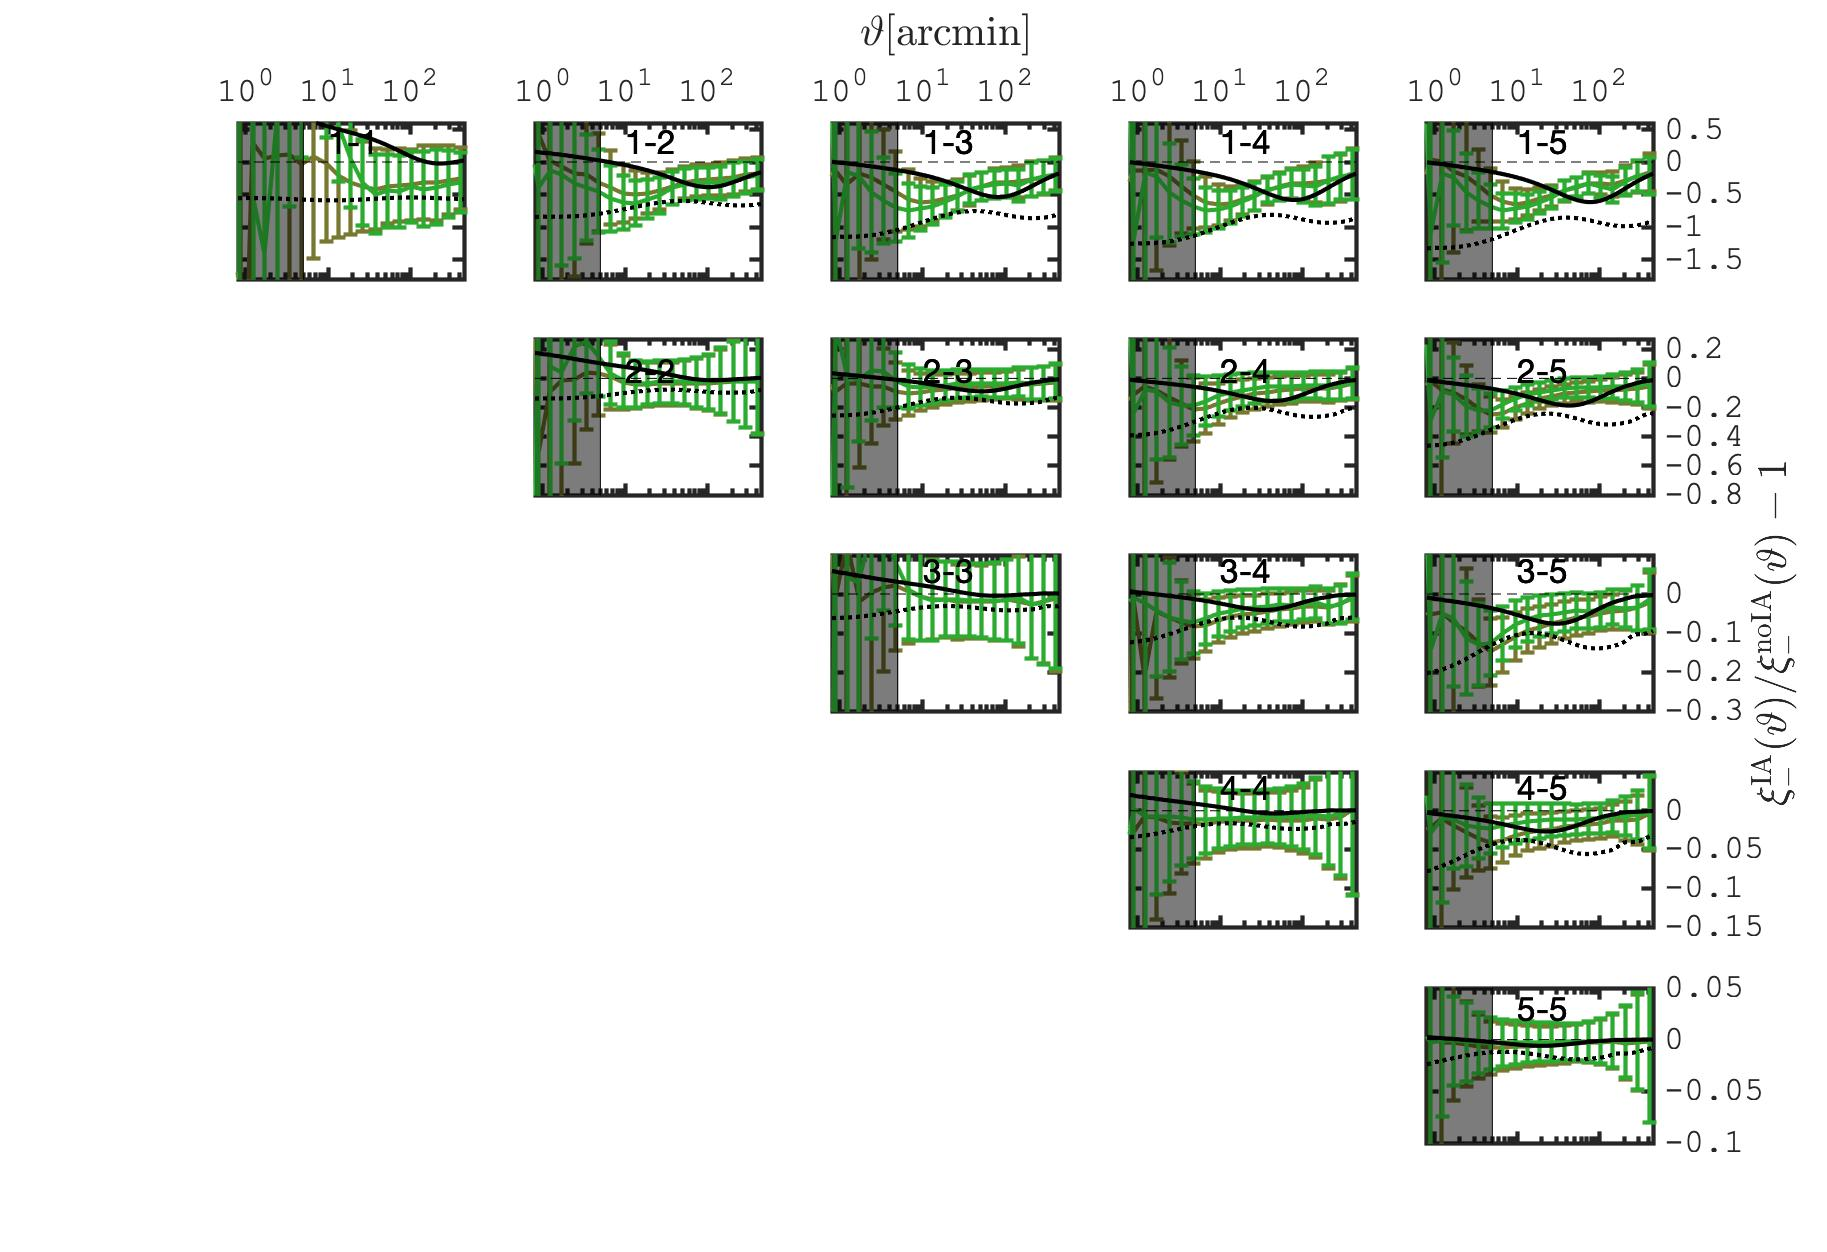
\includegraphics[width=\columnwidth]{graphs/frac_xim_IA1_skysim_deltaTT_srd.jpg}
\caption{Same as Fig. \ref{fig:xi_deltaNLA}, but comparing the TT (brown) and the $\delta$-TT  (green) models, with $A_2=1.0$, $b_{\rm TA}$ = 1.0, and only for smoothing of 0.5$h^{-1}$Mpc. }
\label{fig:xi_deltaTT}
\end{figure*}


To match the theory, we need to apply the following calibration: $\epsilon^{\rm IA, TT}(z<0.5) \rightarrow \epsilon^{\rm IA, TT} /2.5$.

%------------------------------
\subsection{Extended-TT model}
\label{subsec:TT}

See Fig. \ref{fig:xi_deltaTT}

To match the TT theory, we need to apply the following calibration: $\epsilon^{\rm IA, TT}(z<0.5) \rightarrow \epsilon^{\rm IA, TT} /5.0$, followed by $\epsilon^{\rm IA, TT} \rightarrow \epsilon^{\rm IA, TT}/7.0$.

%------------------------------
\subsection{HOD-NLA model}
\label{subsec:HOD}


%--------------
\begin{figure*}
%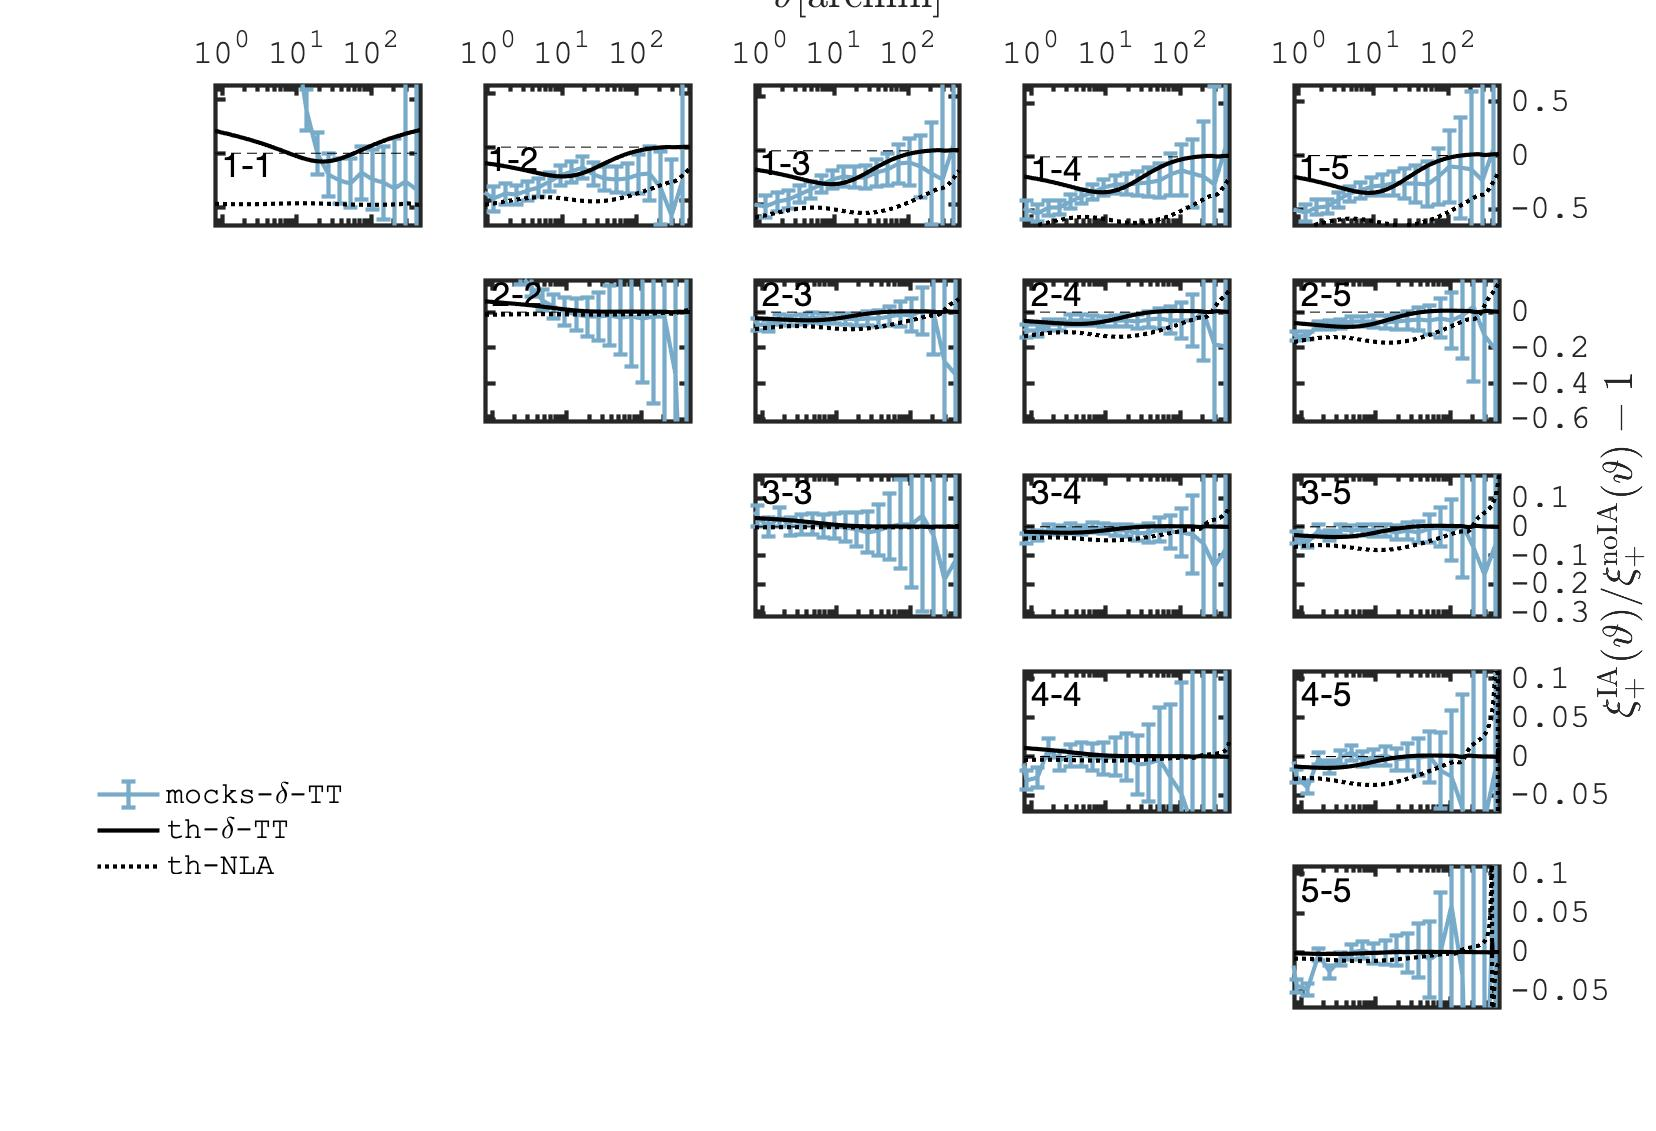
\includegraphics[width=\columnwidth]{graphs/frac_xip_C2_m1_skysim_deltaTT}
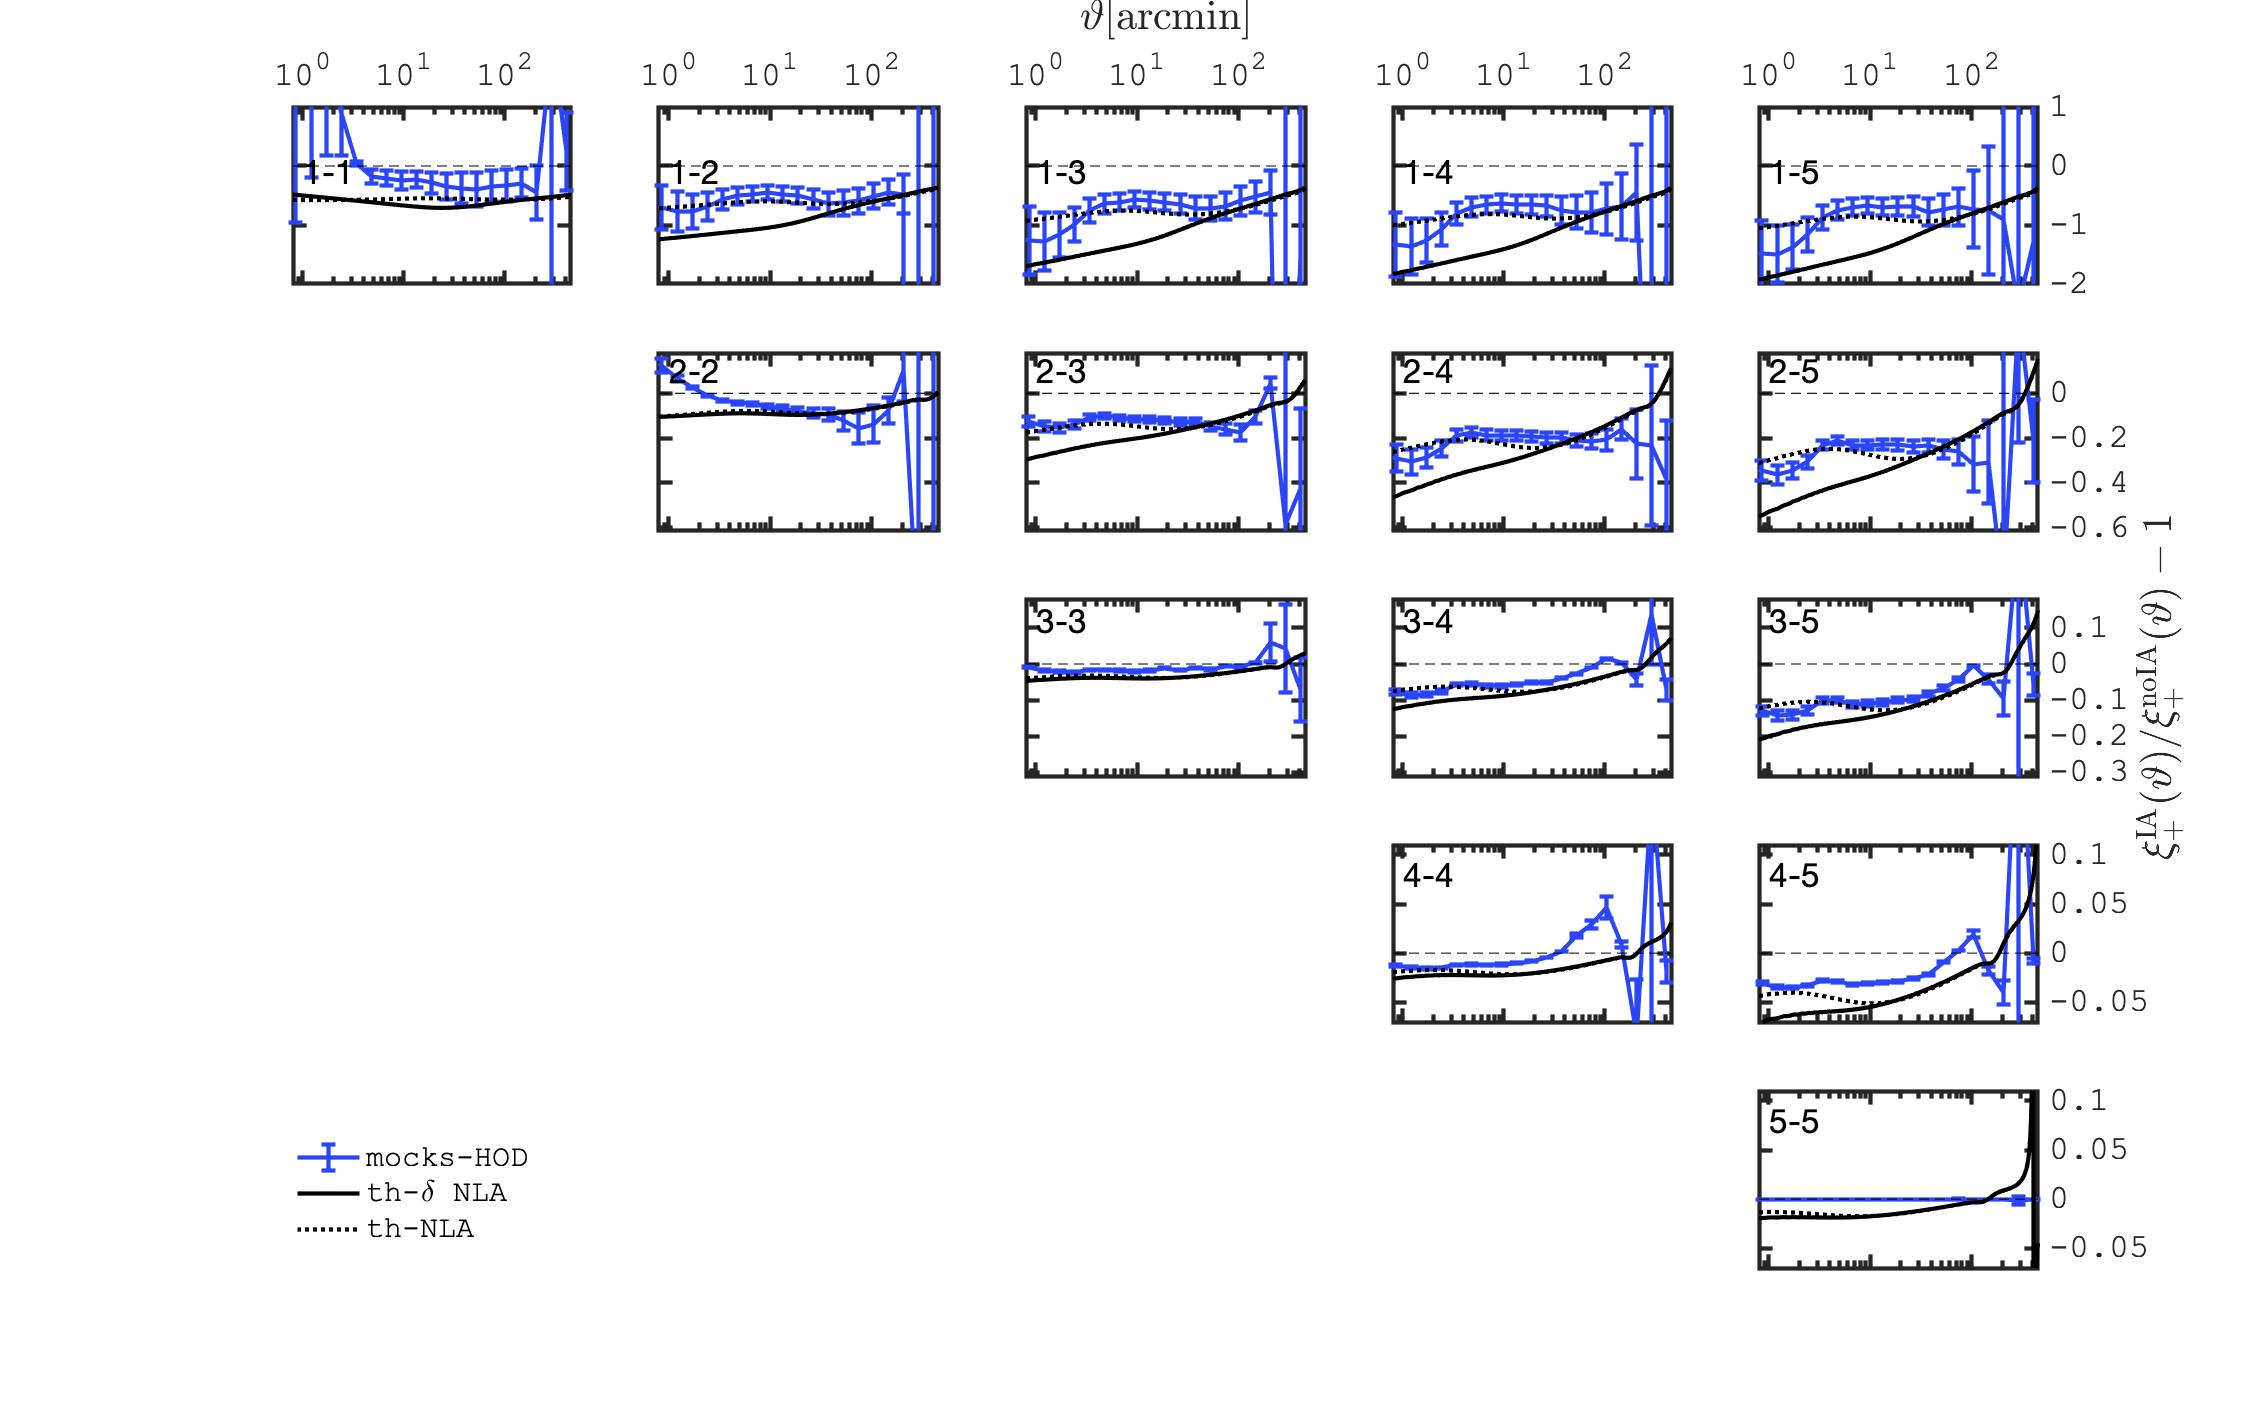
\includegraphics[width=\columnwidth]{graphs/frac_xip_sims_HOD.jpg}
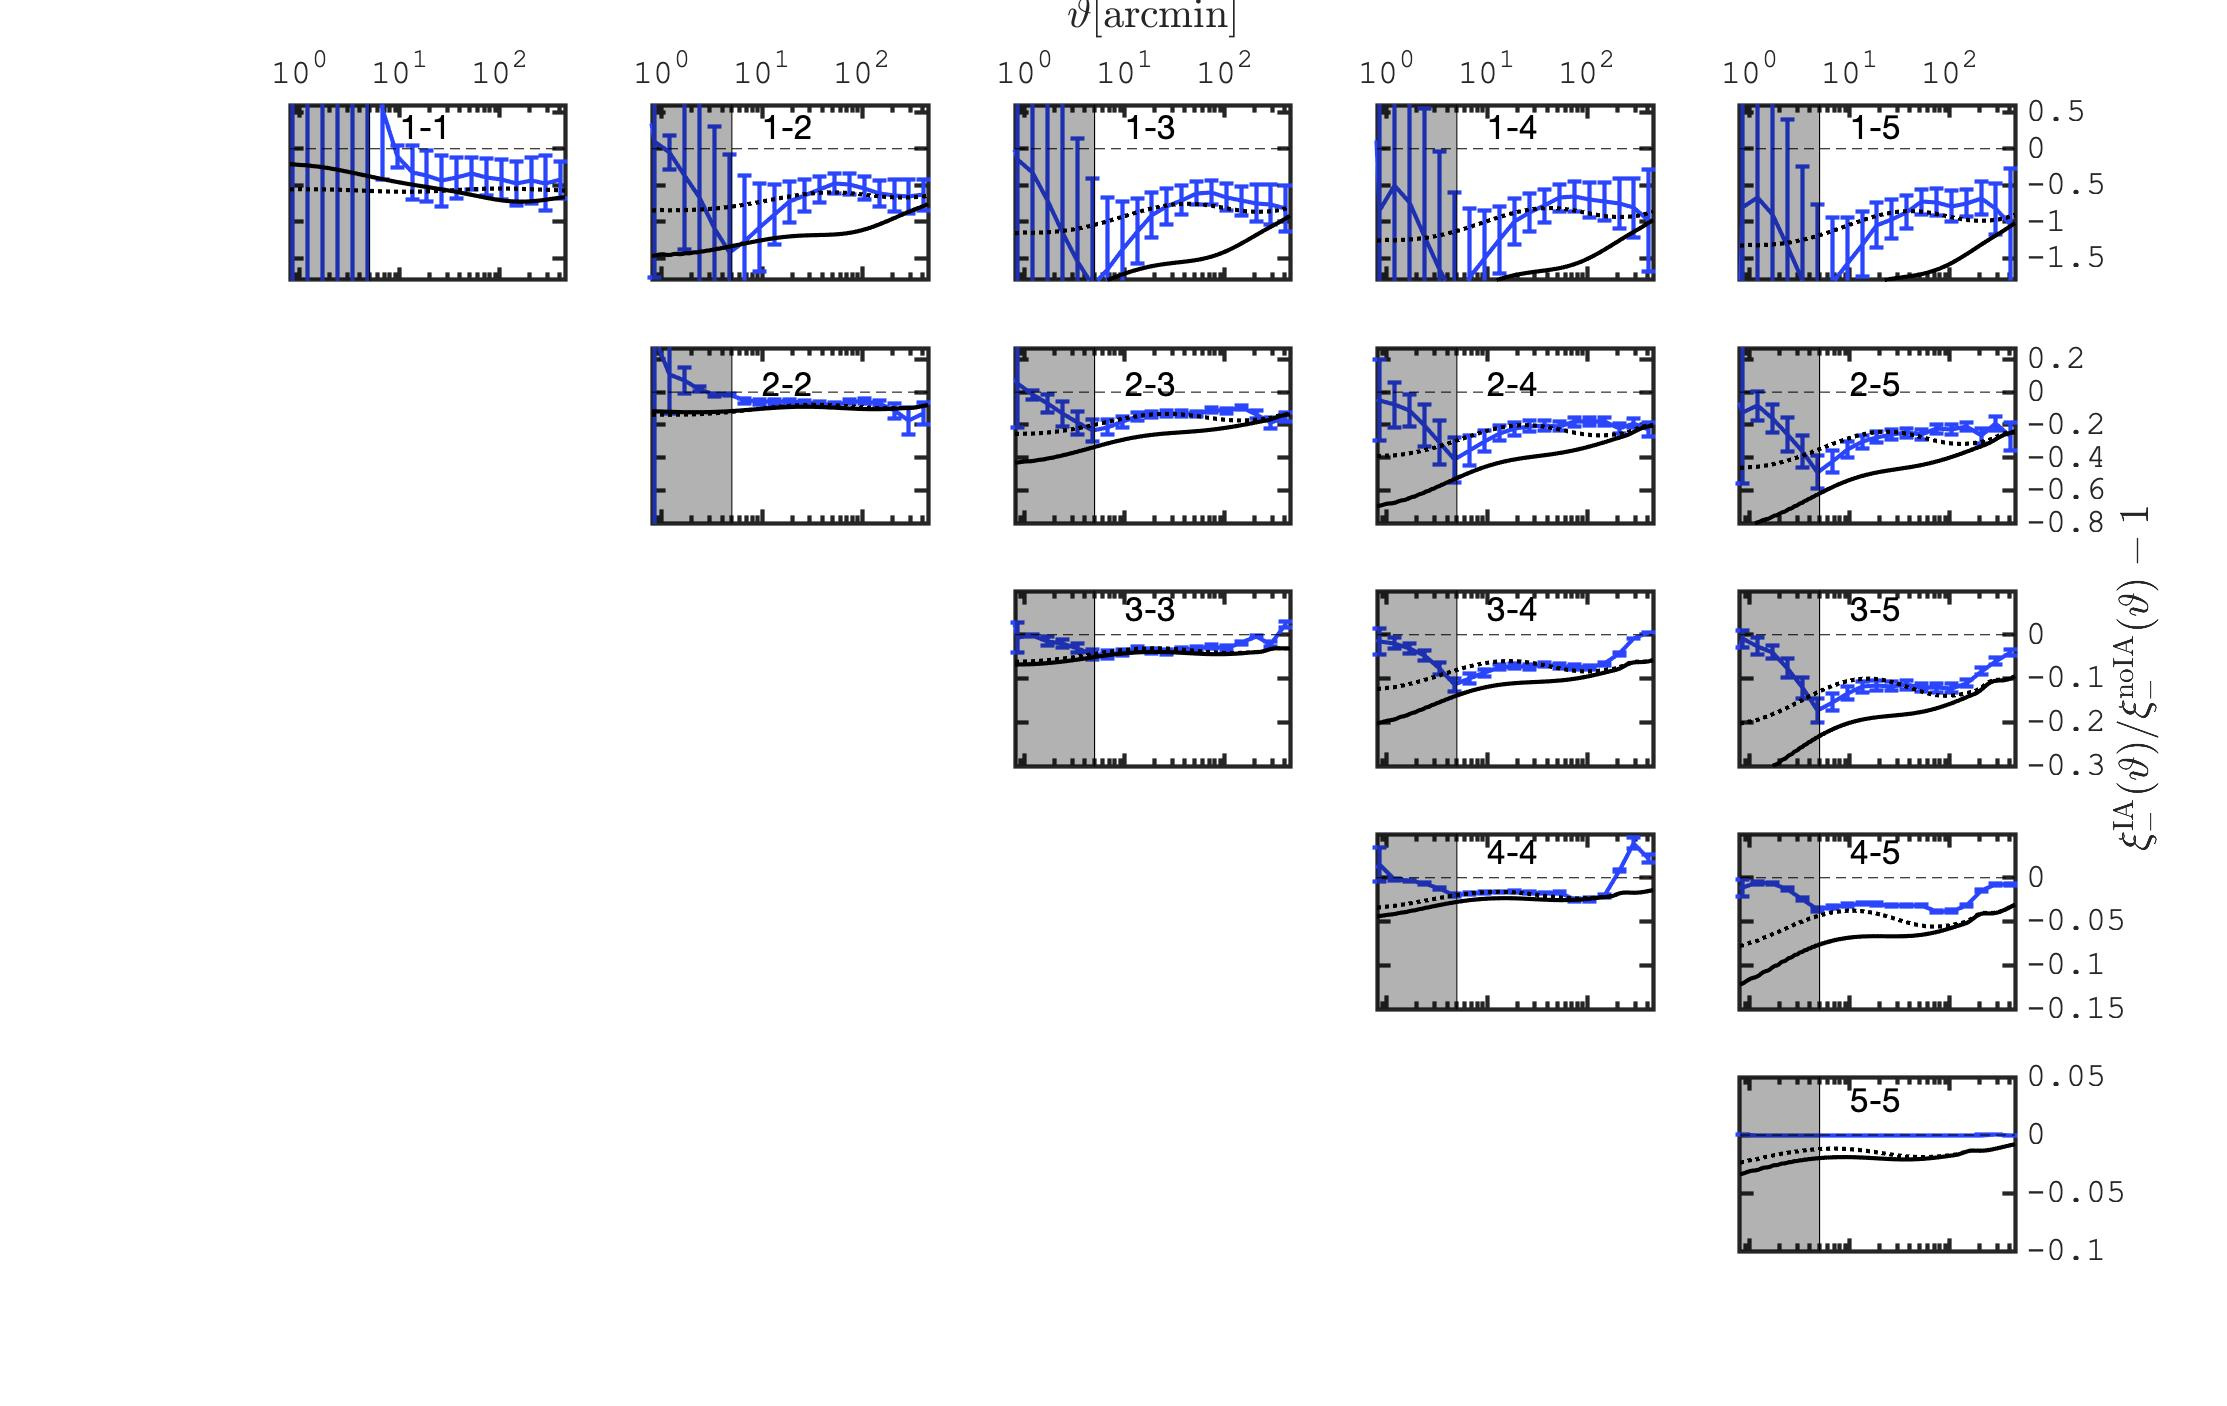
\includegraphics[width=\columnwidth]{graphs/frac_xim_sims_HOD.jpg}
\caption{Same as Fig. \ref{fig:xi_deltaNLA}, but showing the HOD galaxies with shapes linearly coupled with the tidal field. }
\label{fig:xi_hod_nla}
\end{figure*}

%--------------
\begin{figure*}
%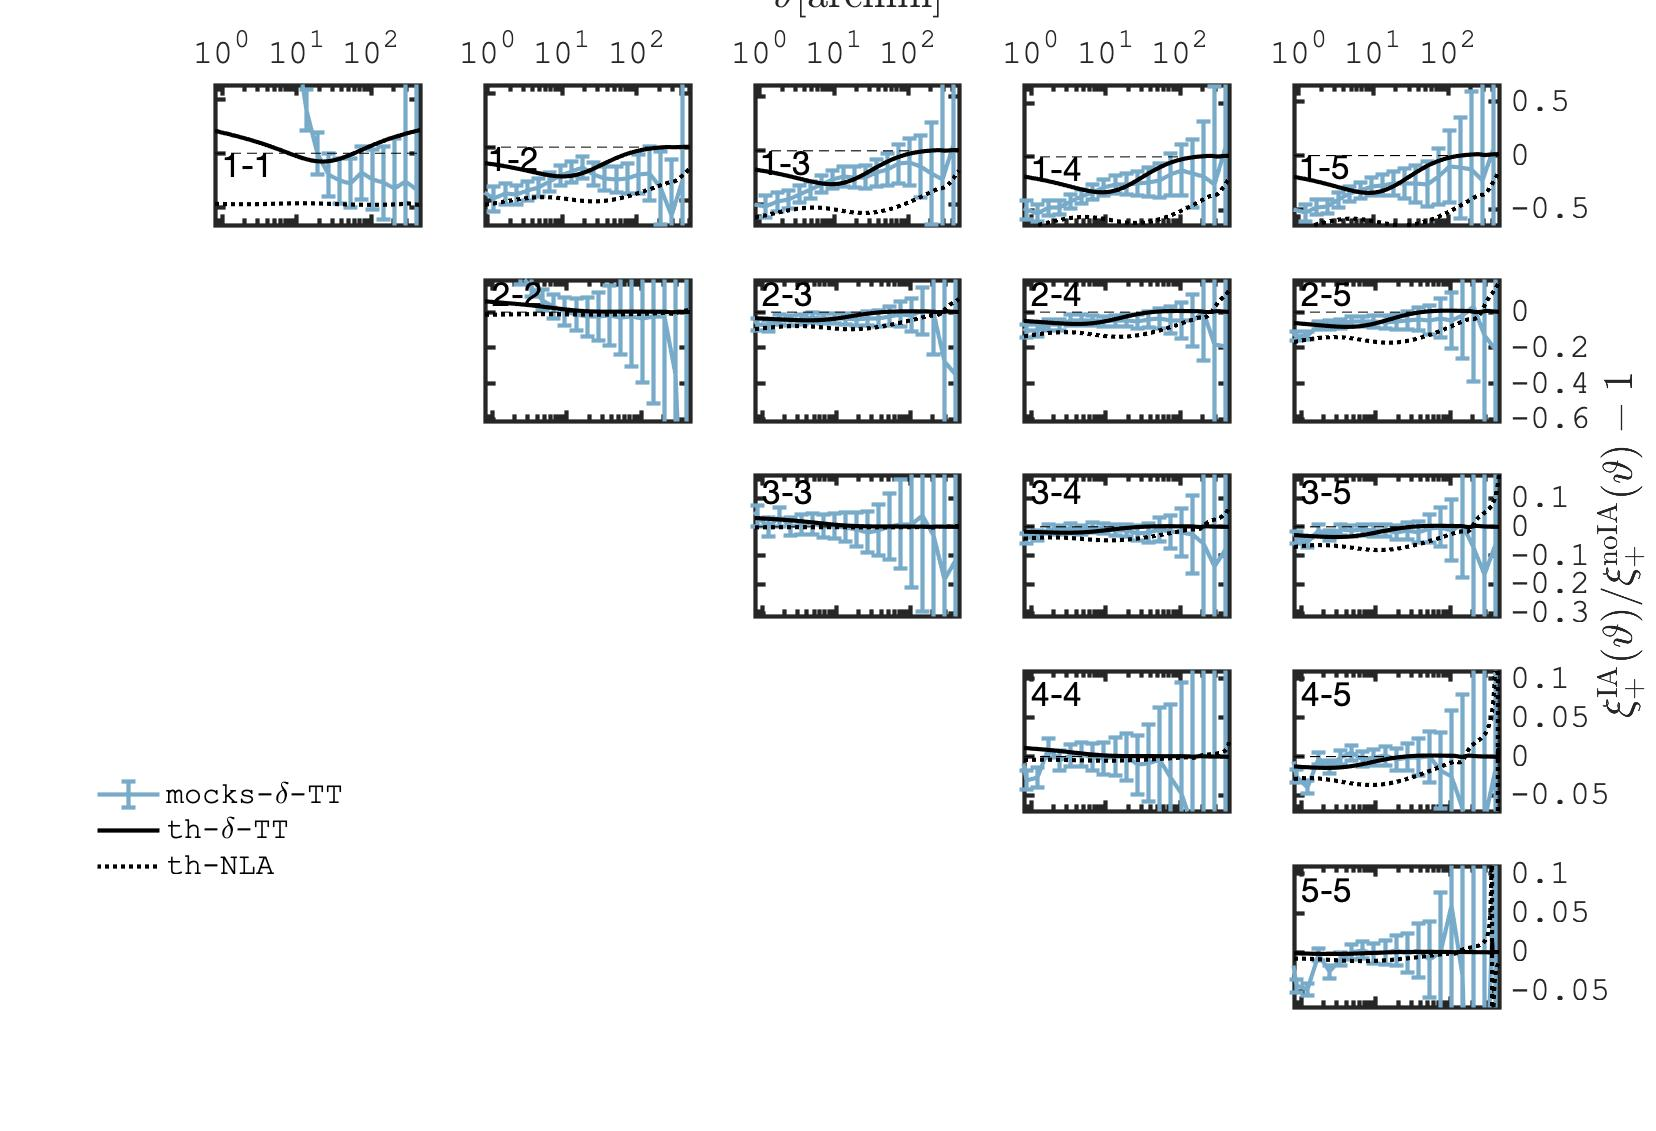
\includegraphics[width=\columnwidth]{graphs/frac_xip_C2_m1_skysim_deltaTT}
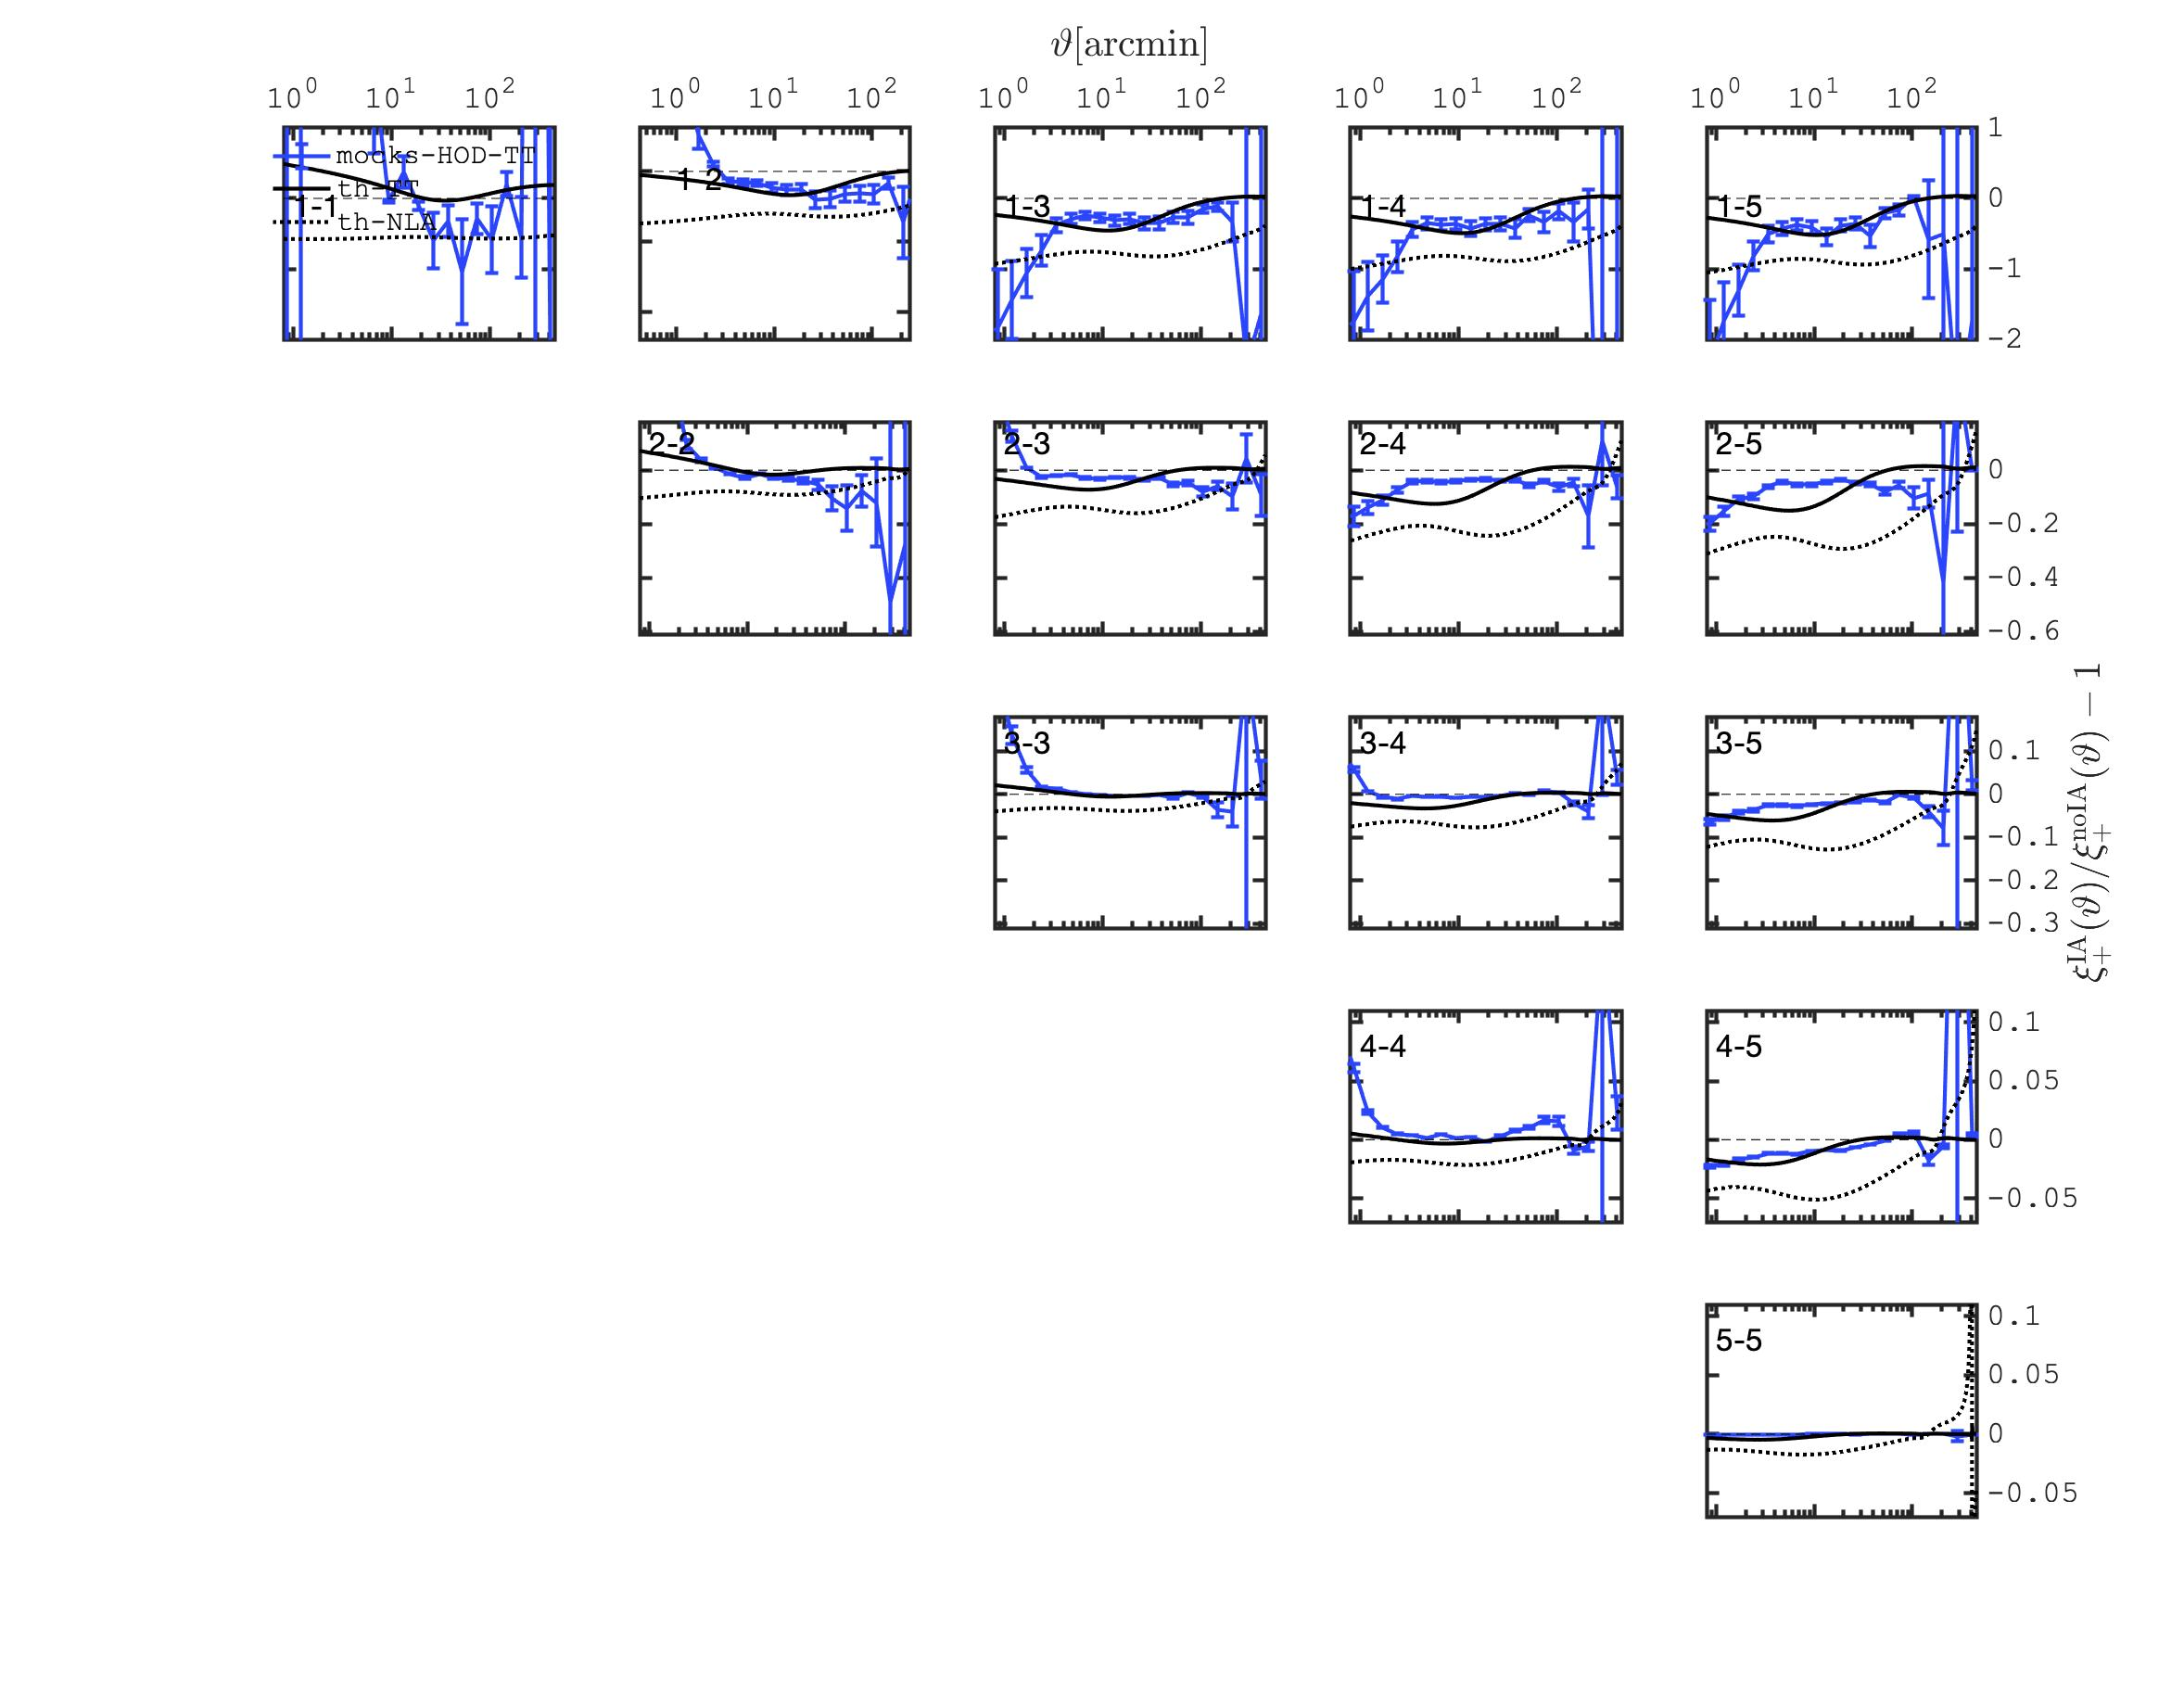
\includegraphics[width=\columnwidth]{graphs/frac_xip_sims_HOD_TT.jpg}
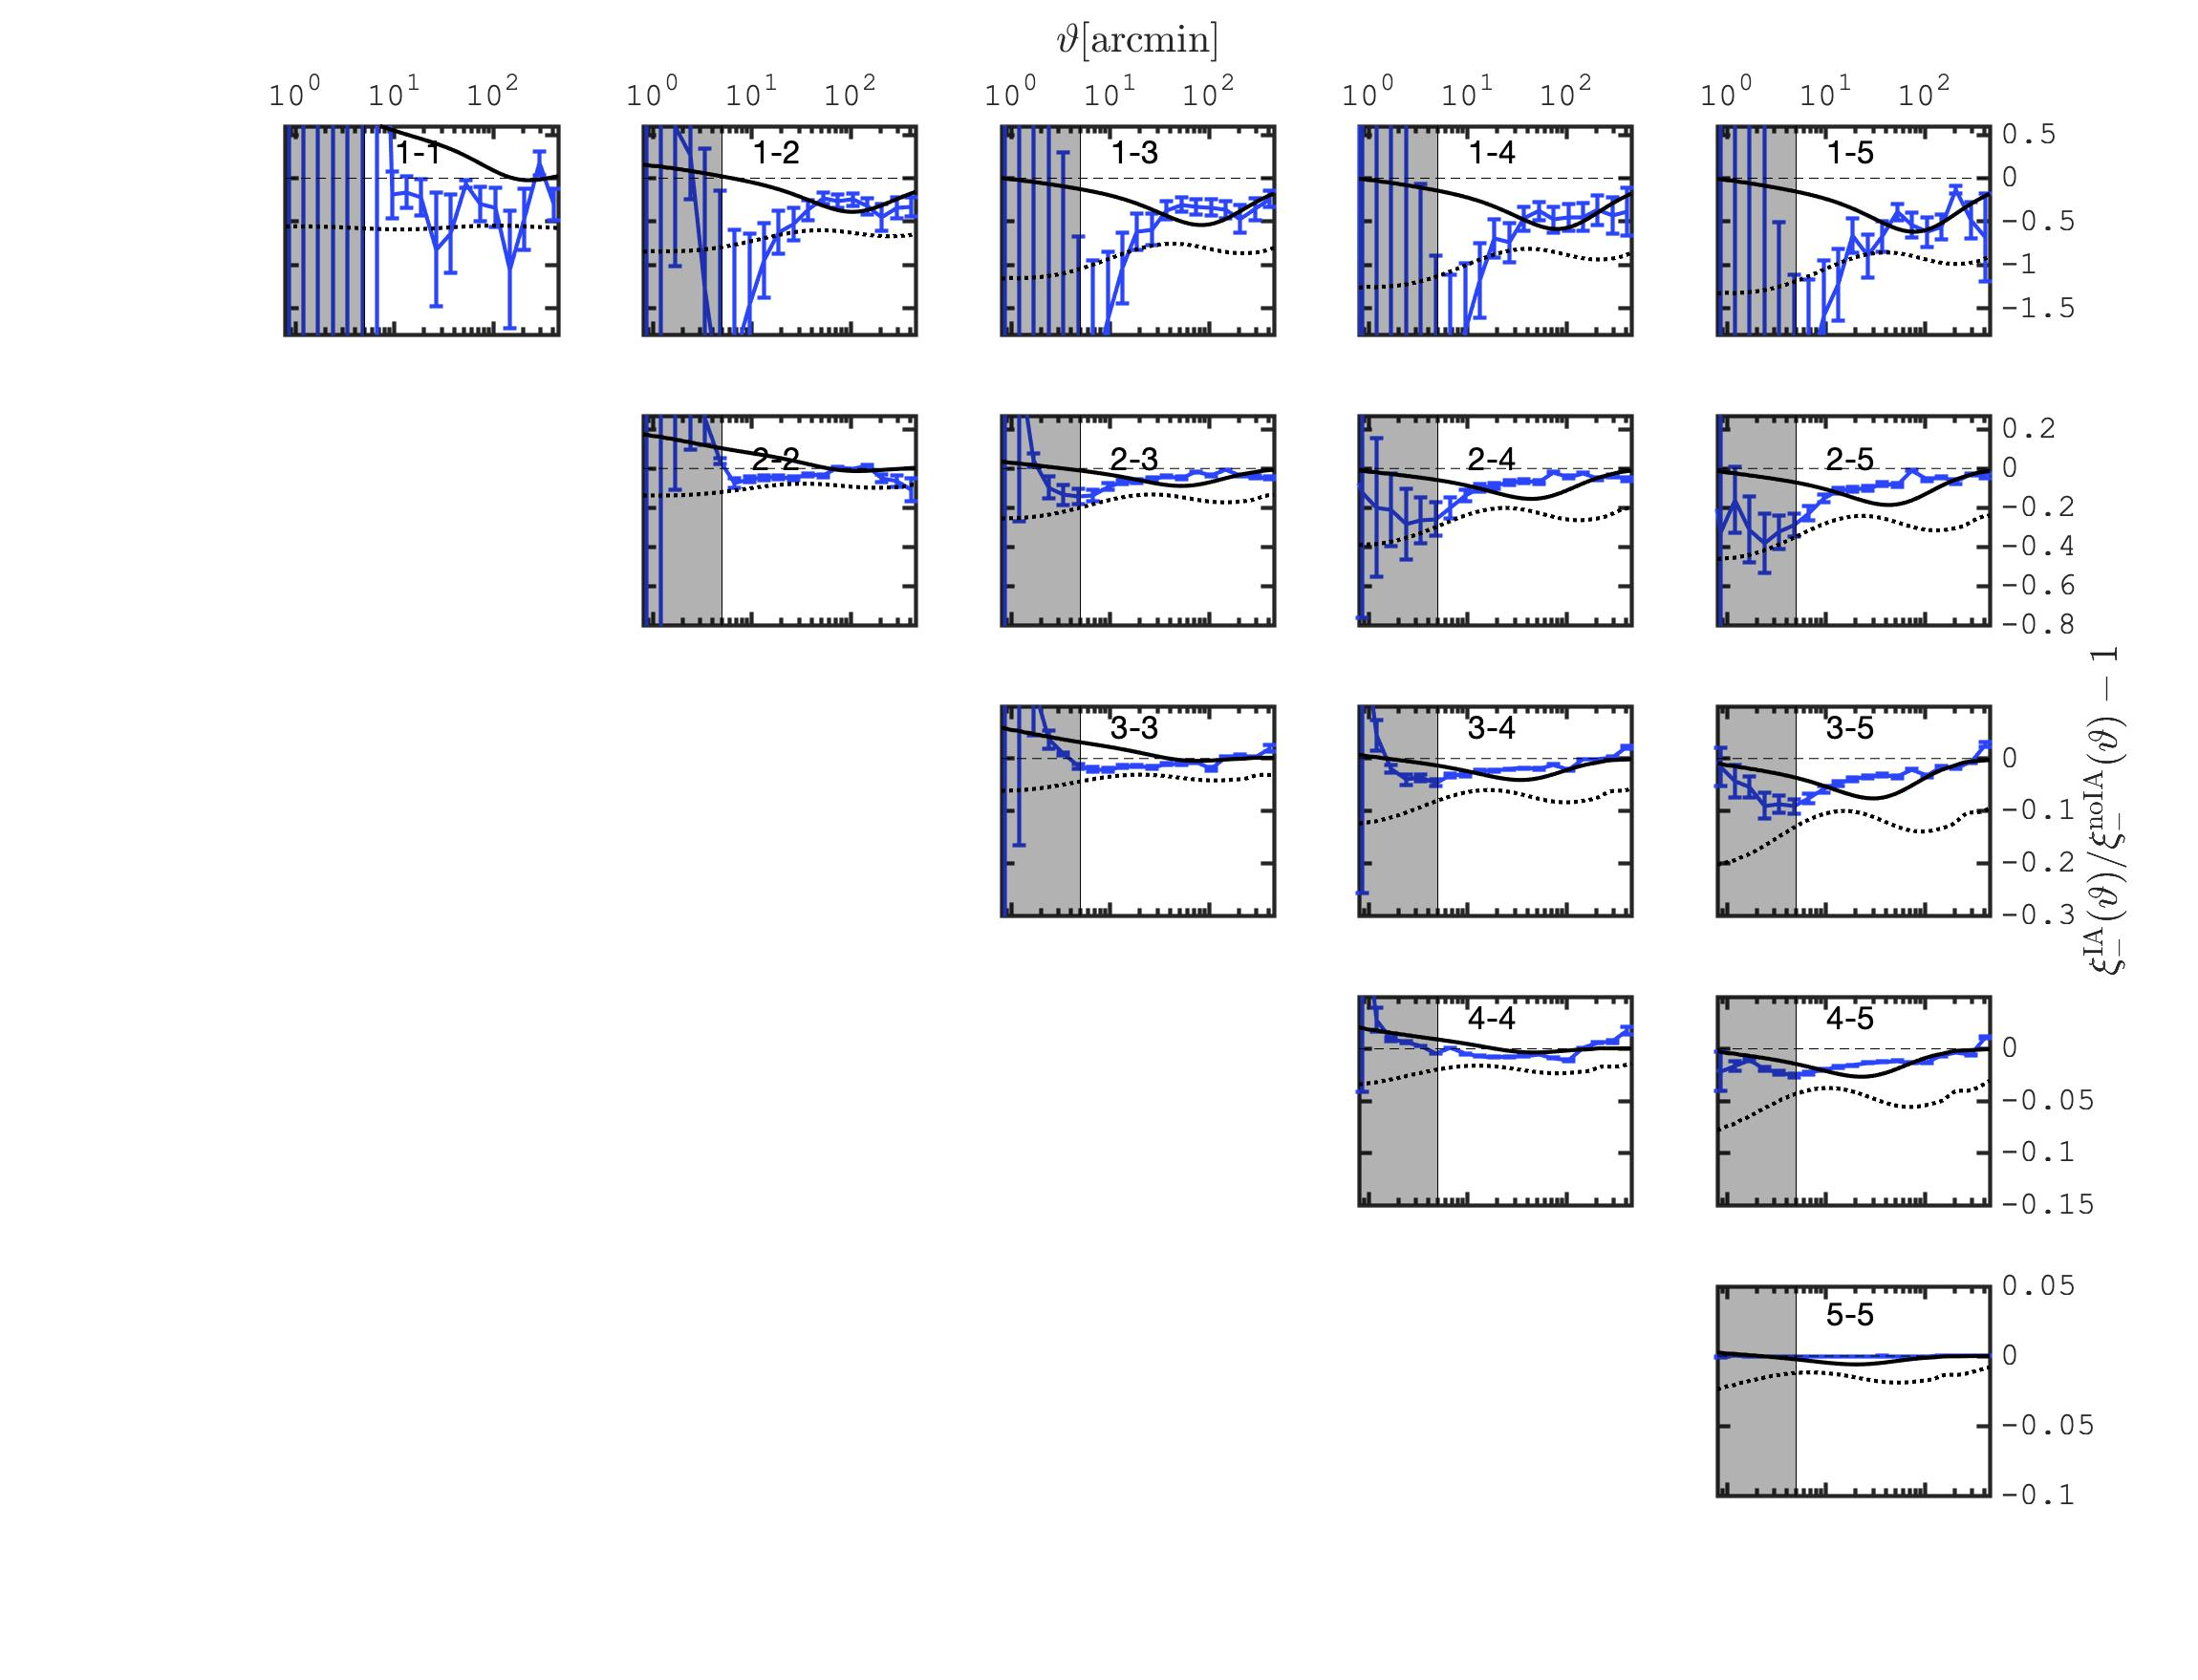
\includegraphics[width=\columnwidth]{graphs/frac_xim_sims_HOD_TT.jpg}
\caption{Same as Fig. \ref{fig:xi_deltaTT}, but showing the HOD galaxies with shapes quadratically coupled with the tidal field. }
\label{fig:xi_hod_tt}
\end{figure*}


The NLA and extended-NLA models respectively assume a null and a linear bias between the source galaxies and the underlying matter field, both of which are approximations to the galaxy dark matter connection.
In fact, galaxies populate dark matter over-densities in a more complex manner \citep{GalaxyPopulationPapers}, which is better described by the Halo Occupation Distribution approach (HOD hereafter).
The largest difference here is that these HOD galaxies are non-linear biased tracers of the matter distribution, which means that a larger number can populate regions of large over-densities, where the tidal fields are generally stronger. 
We therefore expect the impact of IA to be stronger in this case.

We investigate this effect with HOD galaxies extracted from the SkySim5000 simulation \citep{SkySim5000_HOD} \footnote{We used version: {\tt skysim5000\_v1.2}, as detailed in XYZ..}, which are obtained by [...] (mention the TXPipe paper).
Specifically, we select objects over a patch of 732.20 deg$^2$ given by  0$<$RA$<$ 20 and -36.61$<$DEC$<$0, we apply a magnitude cut of mag$_r<$24.8, and further downsample randomly to retain 20\% of the galaxies, 
therefore matching the global galaxy redshift distribution and number density found in the rest of this paper (Eq. \ref{eq:nz}).
The sample is further split into five tomographic bins by using Charlie's magical code (Charlie), resulting in the $n(z)$ presented in Fig. \ref{fig:NzHOD}. 
Compared to the analytical SRD-Y1 presented in Fig. \ref{fig:Nz}, the mean redshifts of the five tomographic bins are shifted by [-0.027, -0.018,  0.003, -0.010,  0.038], respectively.

[{\it To put somewhere?: Since source clustering is a higher order effect in cosmic shear, the measured $\xi_{\pm}$ from these three mocks (random, $b_{\rm TA}=1.0$ and $b_{\rm TA}=2.0$) show negligible differences ({\it to quantify and cite}). 
In contrast, the impact on the IA contamination is significant and can double the secondary signal in certain circumstances. 
The main explanation for this is that while clustered sources are uncorrelated with the foreground matter responsible for the lensing signal, the high-density regions they live are also subject to the largest tidal fields. 
}]


\subsection{Validation with full inference}
 \label{sec:inference}
\begin{figure}
%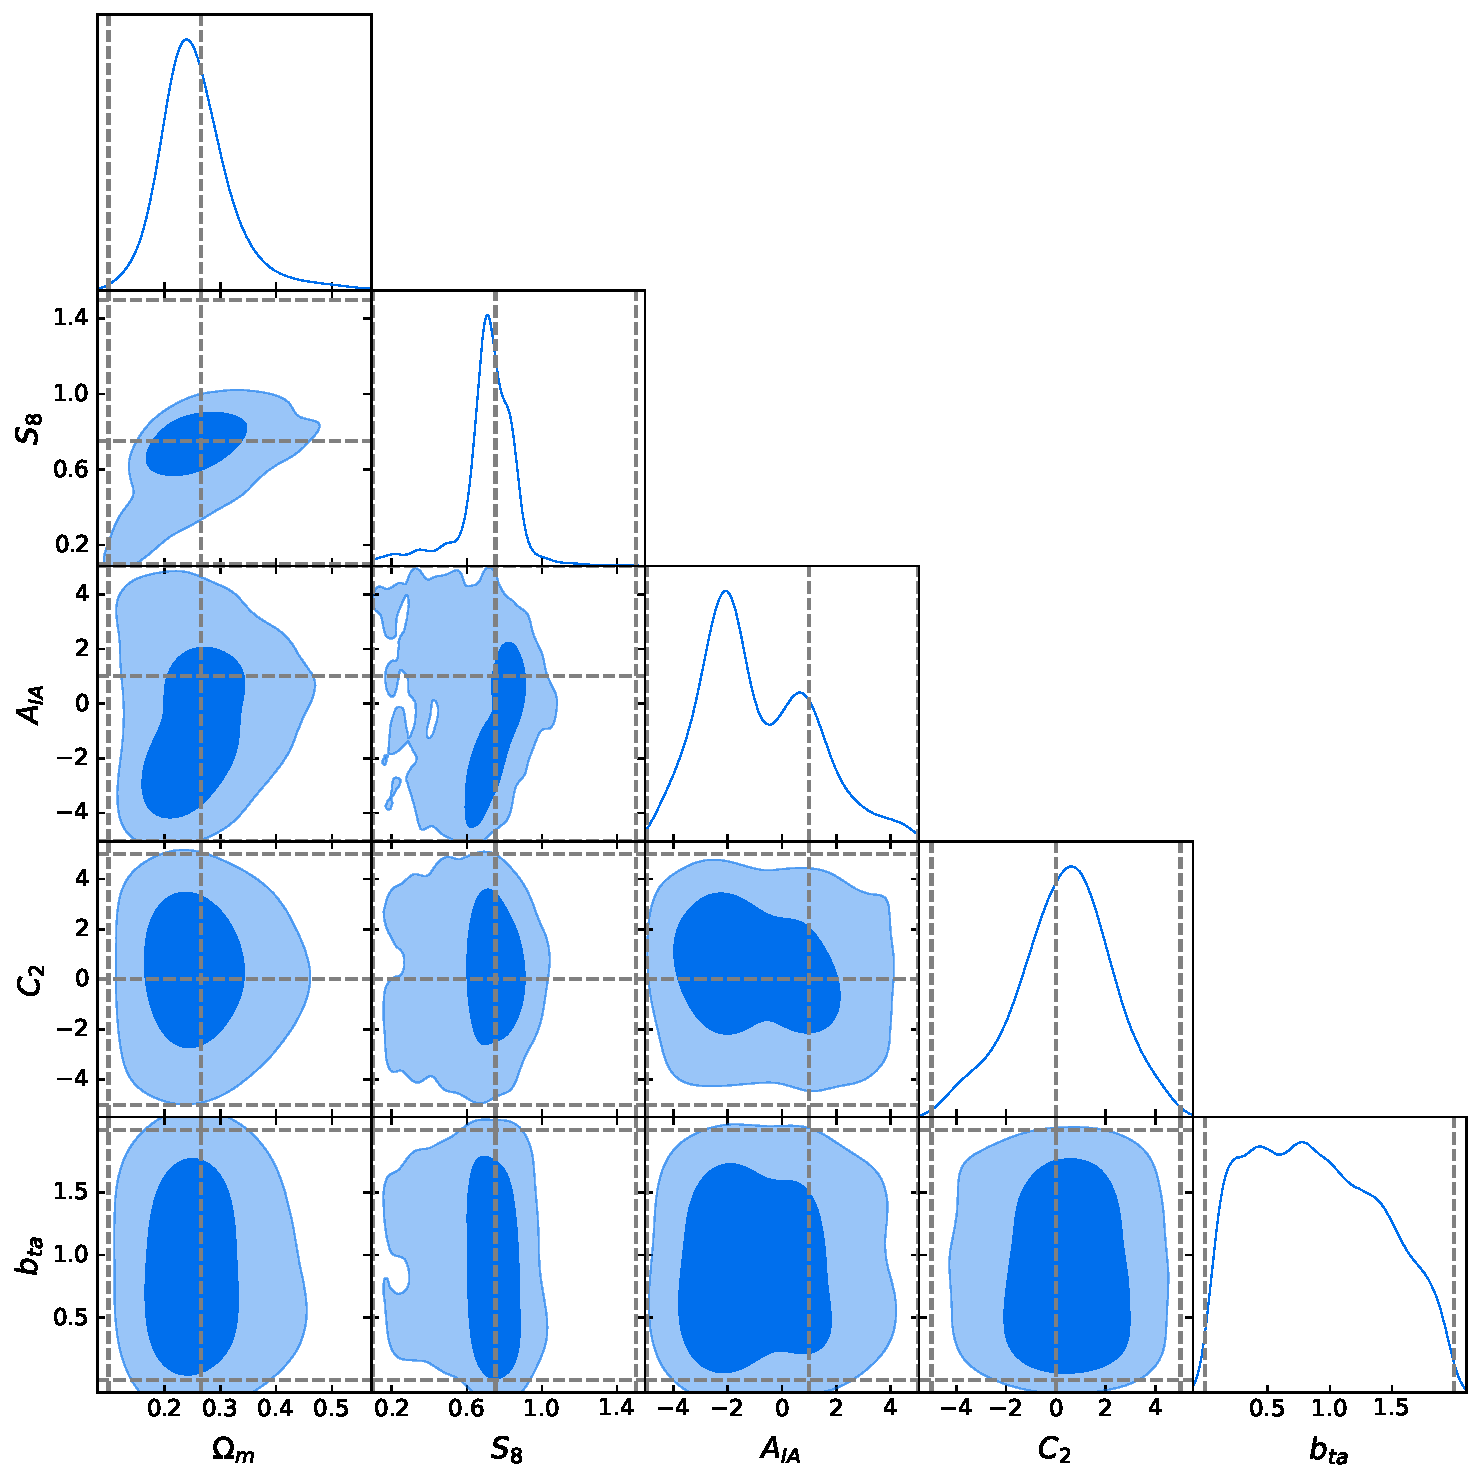
\includegraphics[width=\columnwidth]{graphs/triangle_nla_5D.pdf}
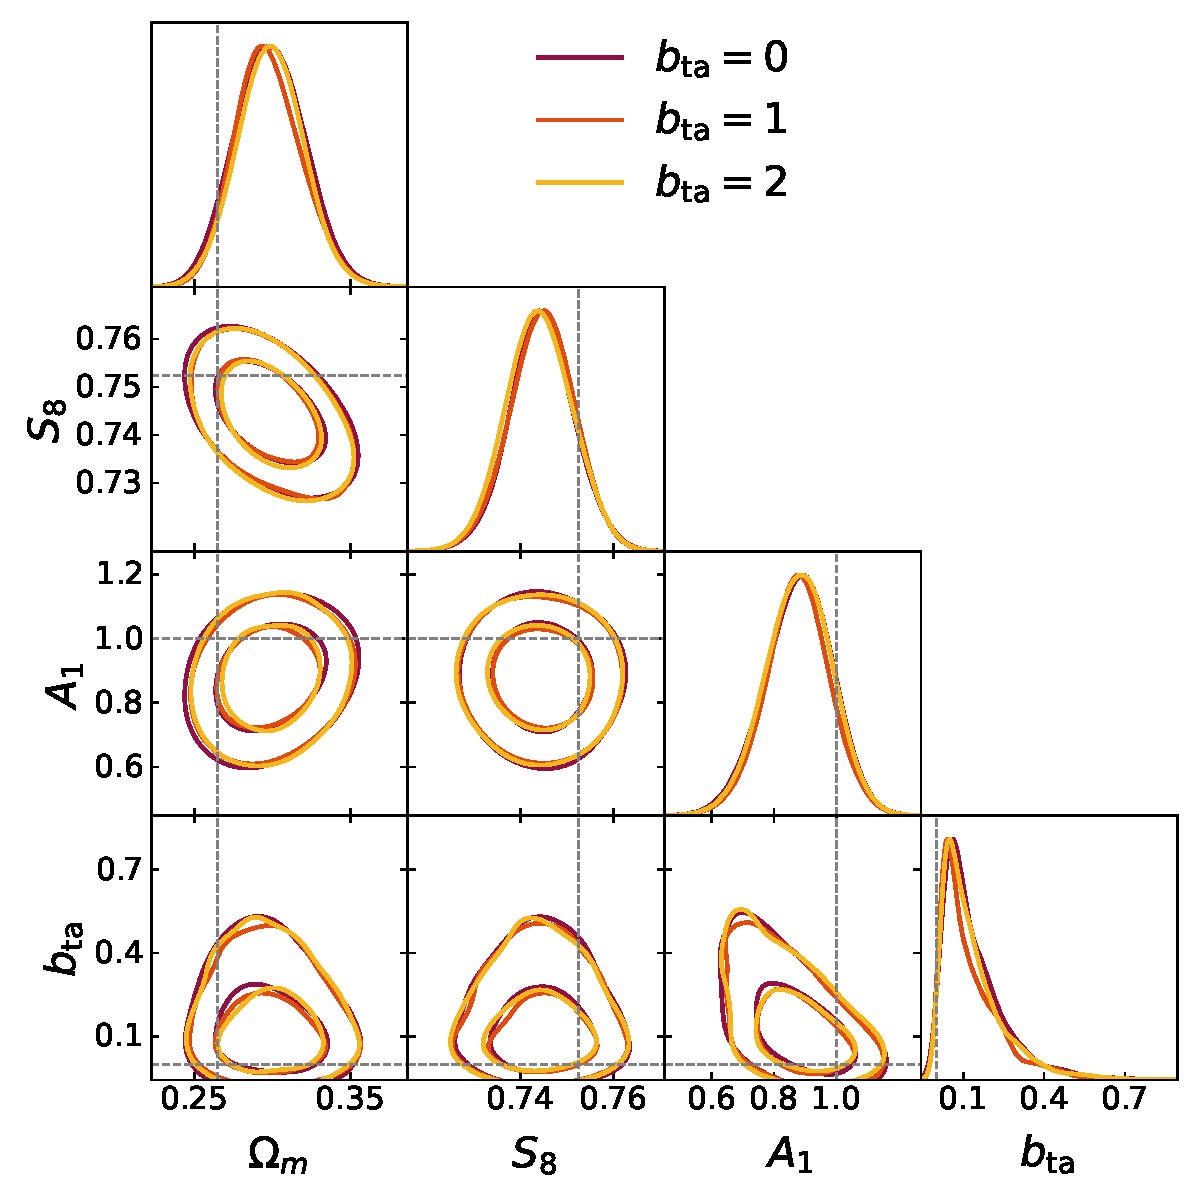
\includegraphics[width=\columnwidth]{graphs/triangle_bta_sweep.pdf}
\caption{Cosmological inference from the NLA-infused simulations, analysed the extended-NLA model. 
The cross-hairs represent the truth as fixed in the {\it Outer Rim} $N$-body simulations \citep{OuterRim}. \niko{we should remove this fig, it is now irrelevant. or i can redo it with the new scale cuts}}
\label{fig:triangle_nla}
\end{figure}
priors, {\sc CosmoSIS}, Takahashi $P(k)$, etc.

\begin{figure}
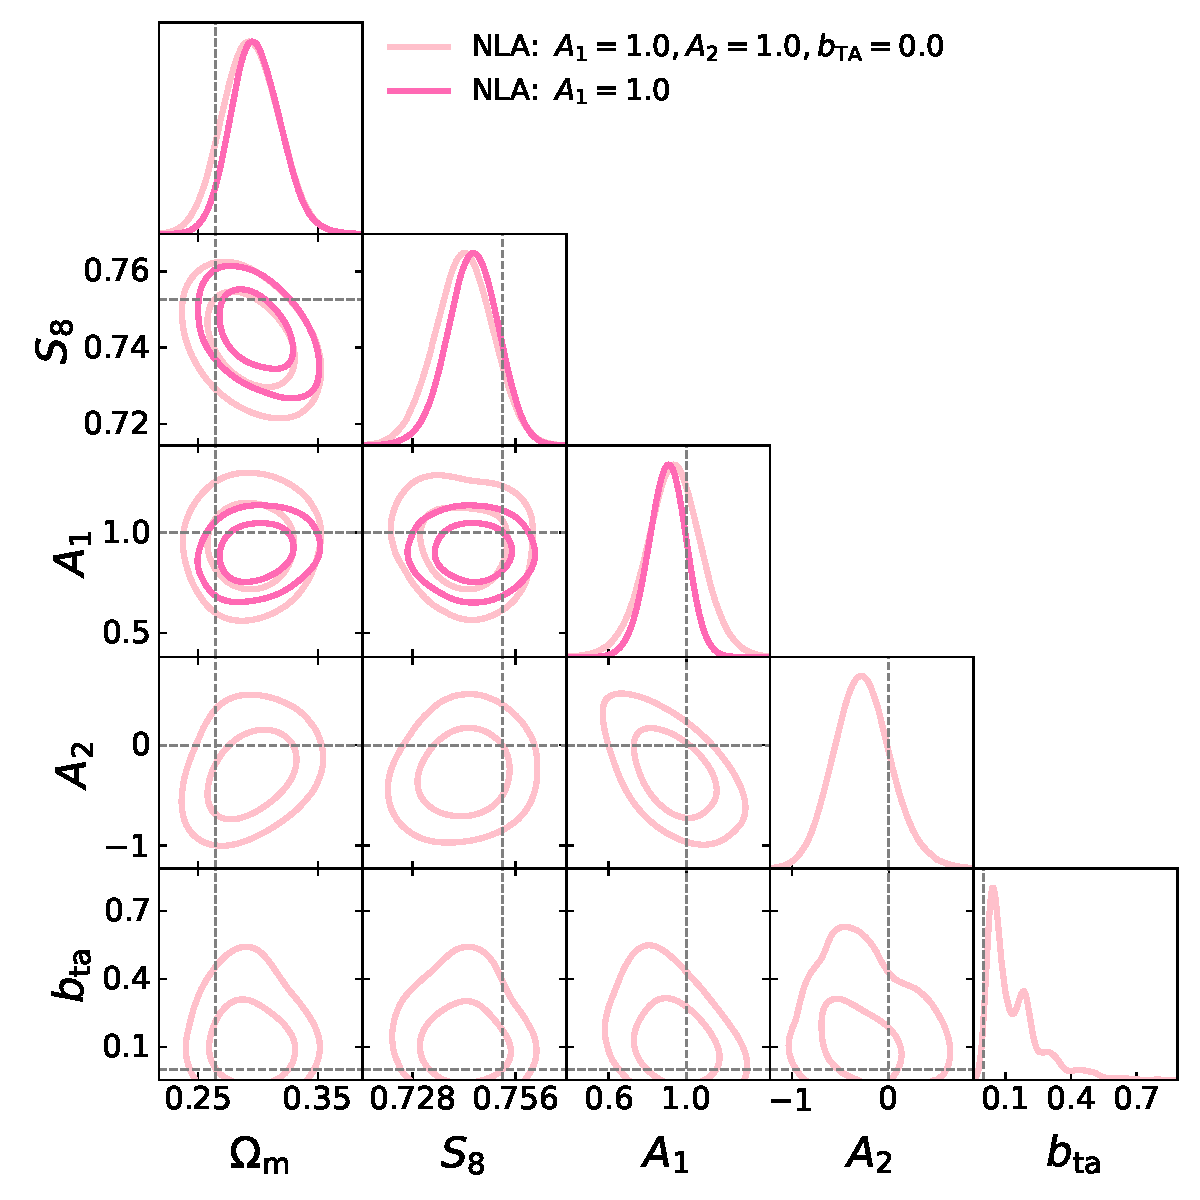
\includegraphics[width=\columnwidth]{graphs/NLA_1_0_0.pdf}
\caption{Cosmological inference from the NLA-infused simulations, with all 3 IA parameters varied (light pink) and with varying A1 only (dark pink).
The cross-hairs represent the truth as fixed in the {\it Outer Rim} $N$-body simulations \citep{OuterRim}.}
\label{fig:corner_nla_all_ia_params}
\end{figure}



\begin{figure}
%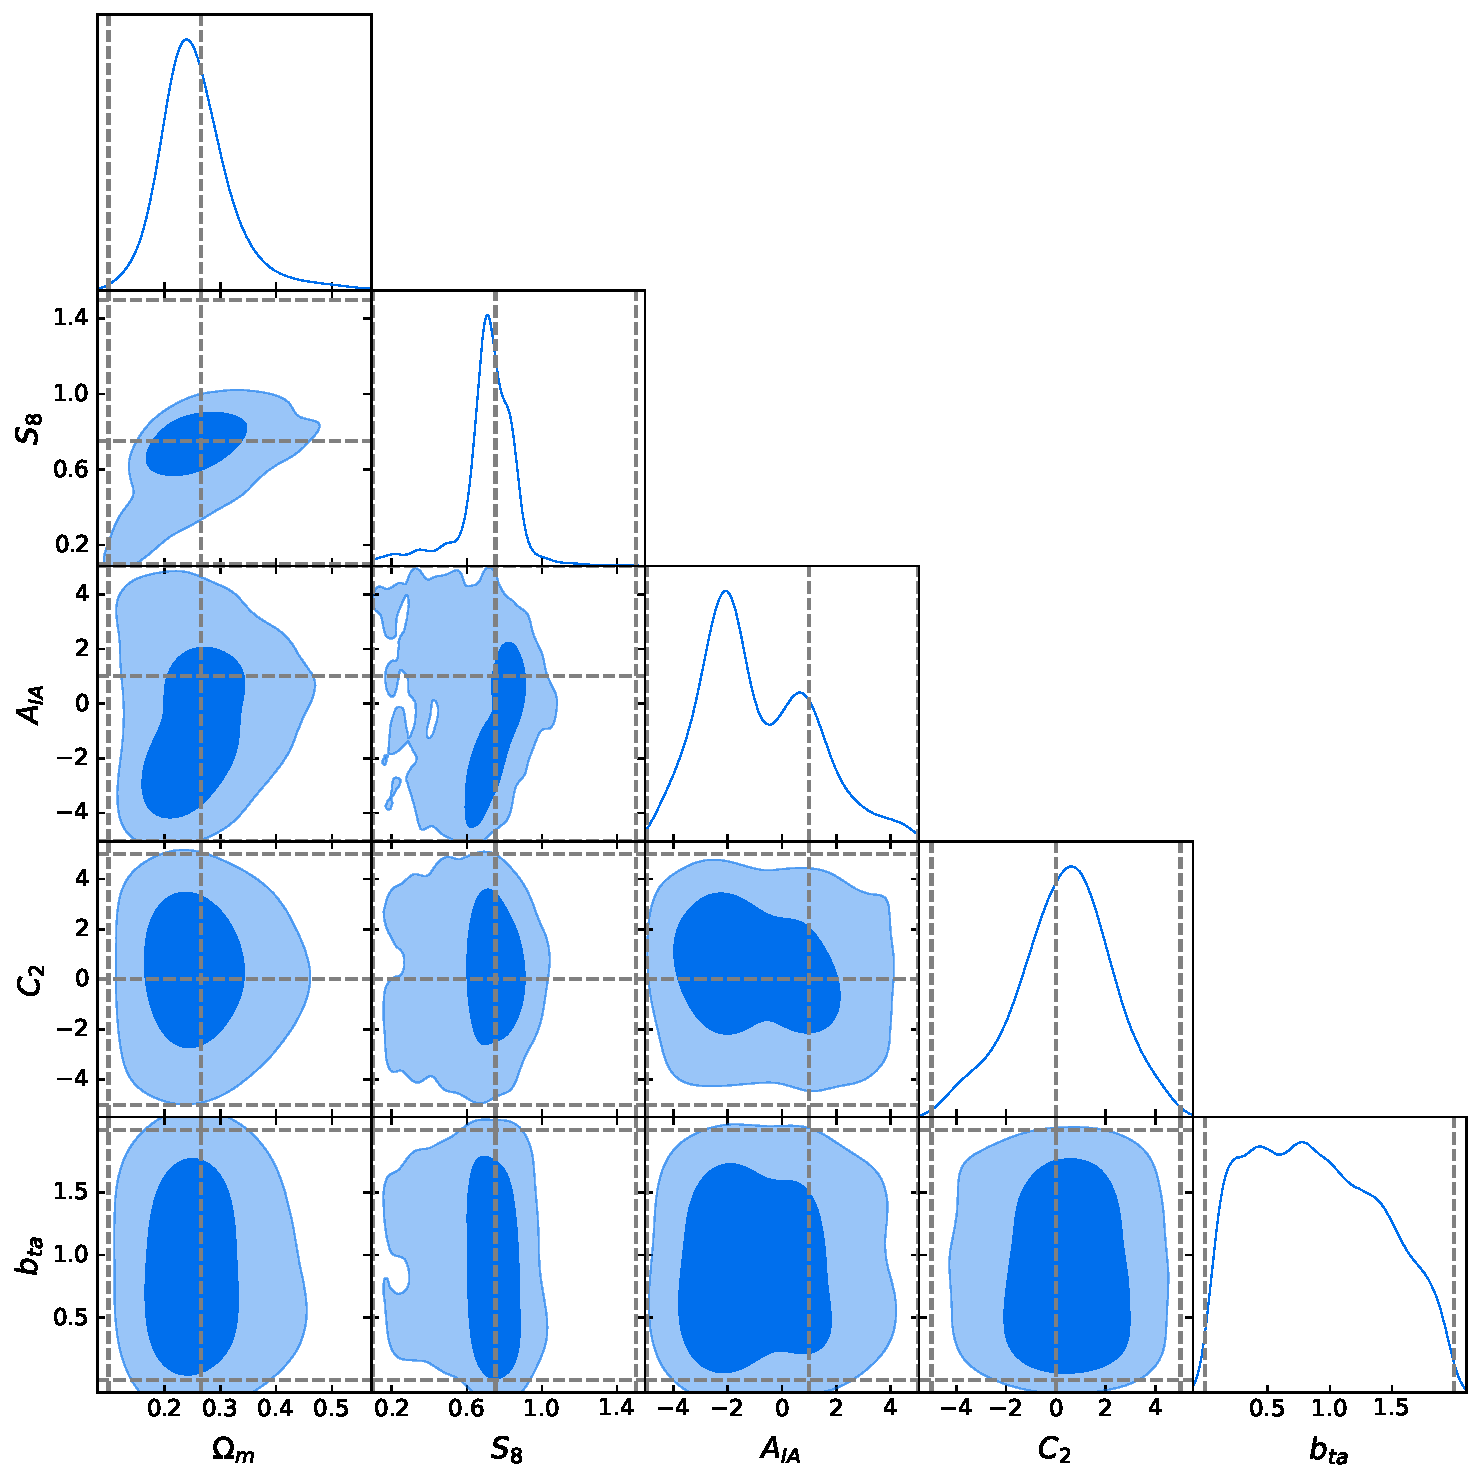
\includegraphics[width=\columnwidth]{graphs/triangle_nla_5D.pdf}
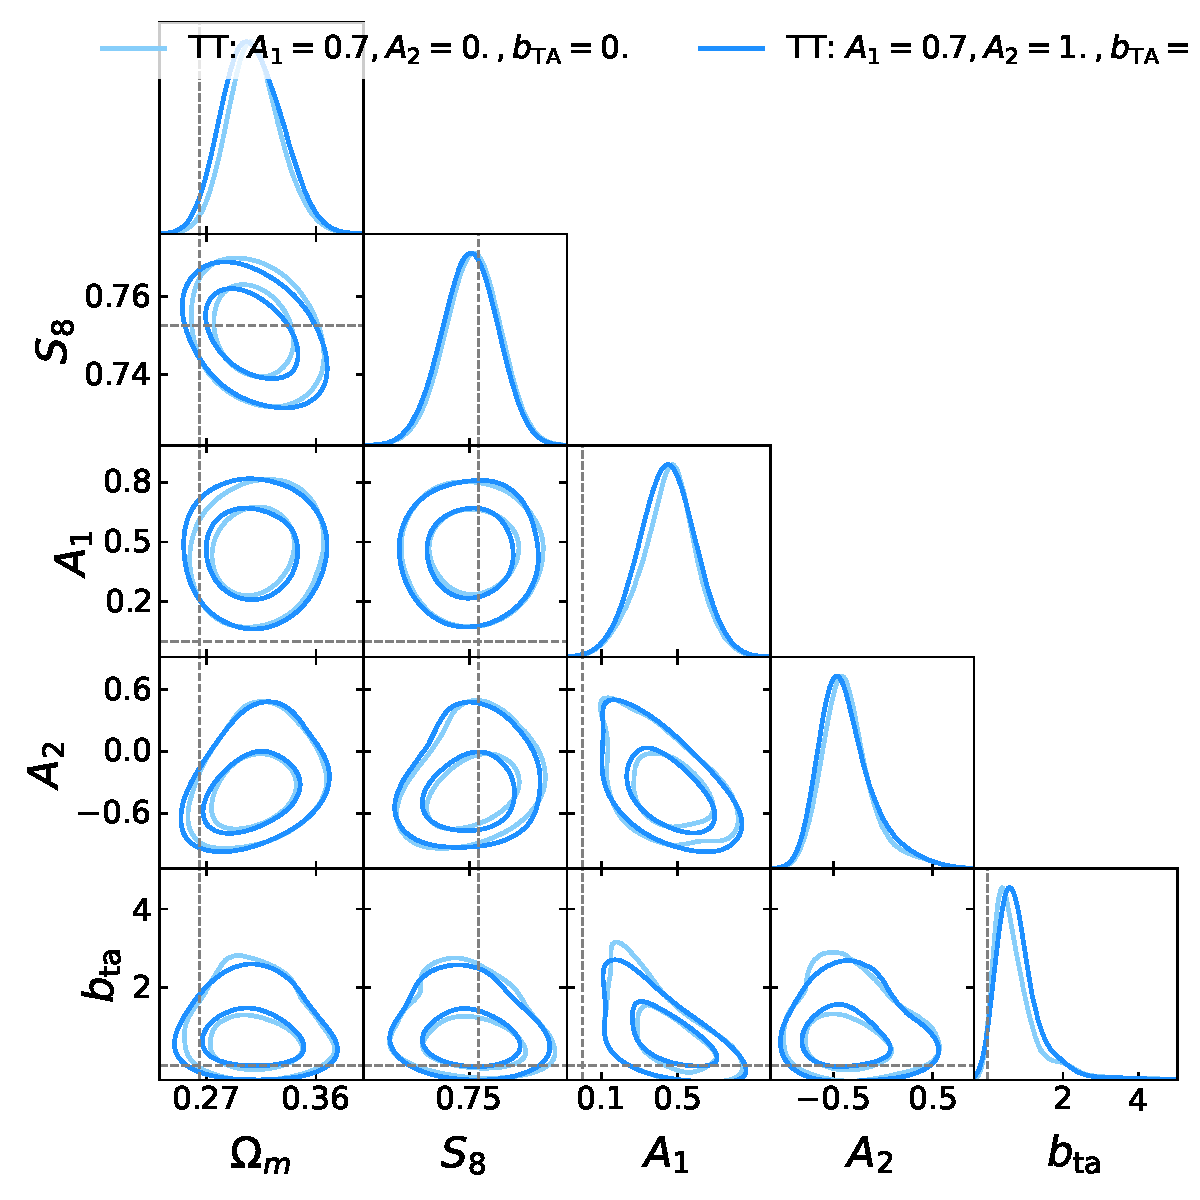
\includegraphics[width=\columnwidth]{graphs/TT_allsweep.pdf}
\caption{Cosmological inference from the TT-infused simulations, with all 3 IA params varied. The cross-hairs represent the truth as fixed in the {\it Outer Rim} $N$-body simulations \citep{OuterRim}.\niko{we should remove this fig, it is now irrelevant. or i can redo it with the new scale cuts}}
\label{fig:triangle_tt_all_ia_params}
\end{figure}

\begin{figure}
%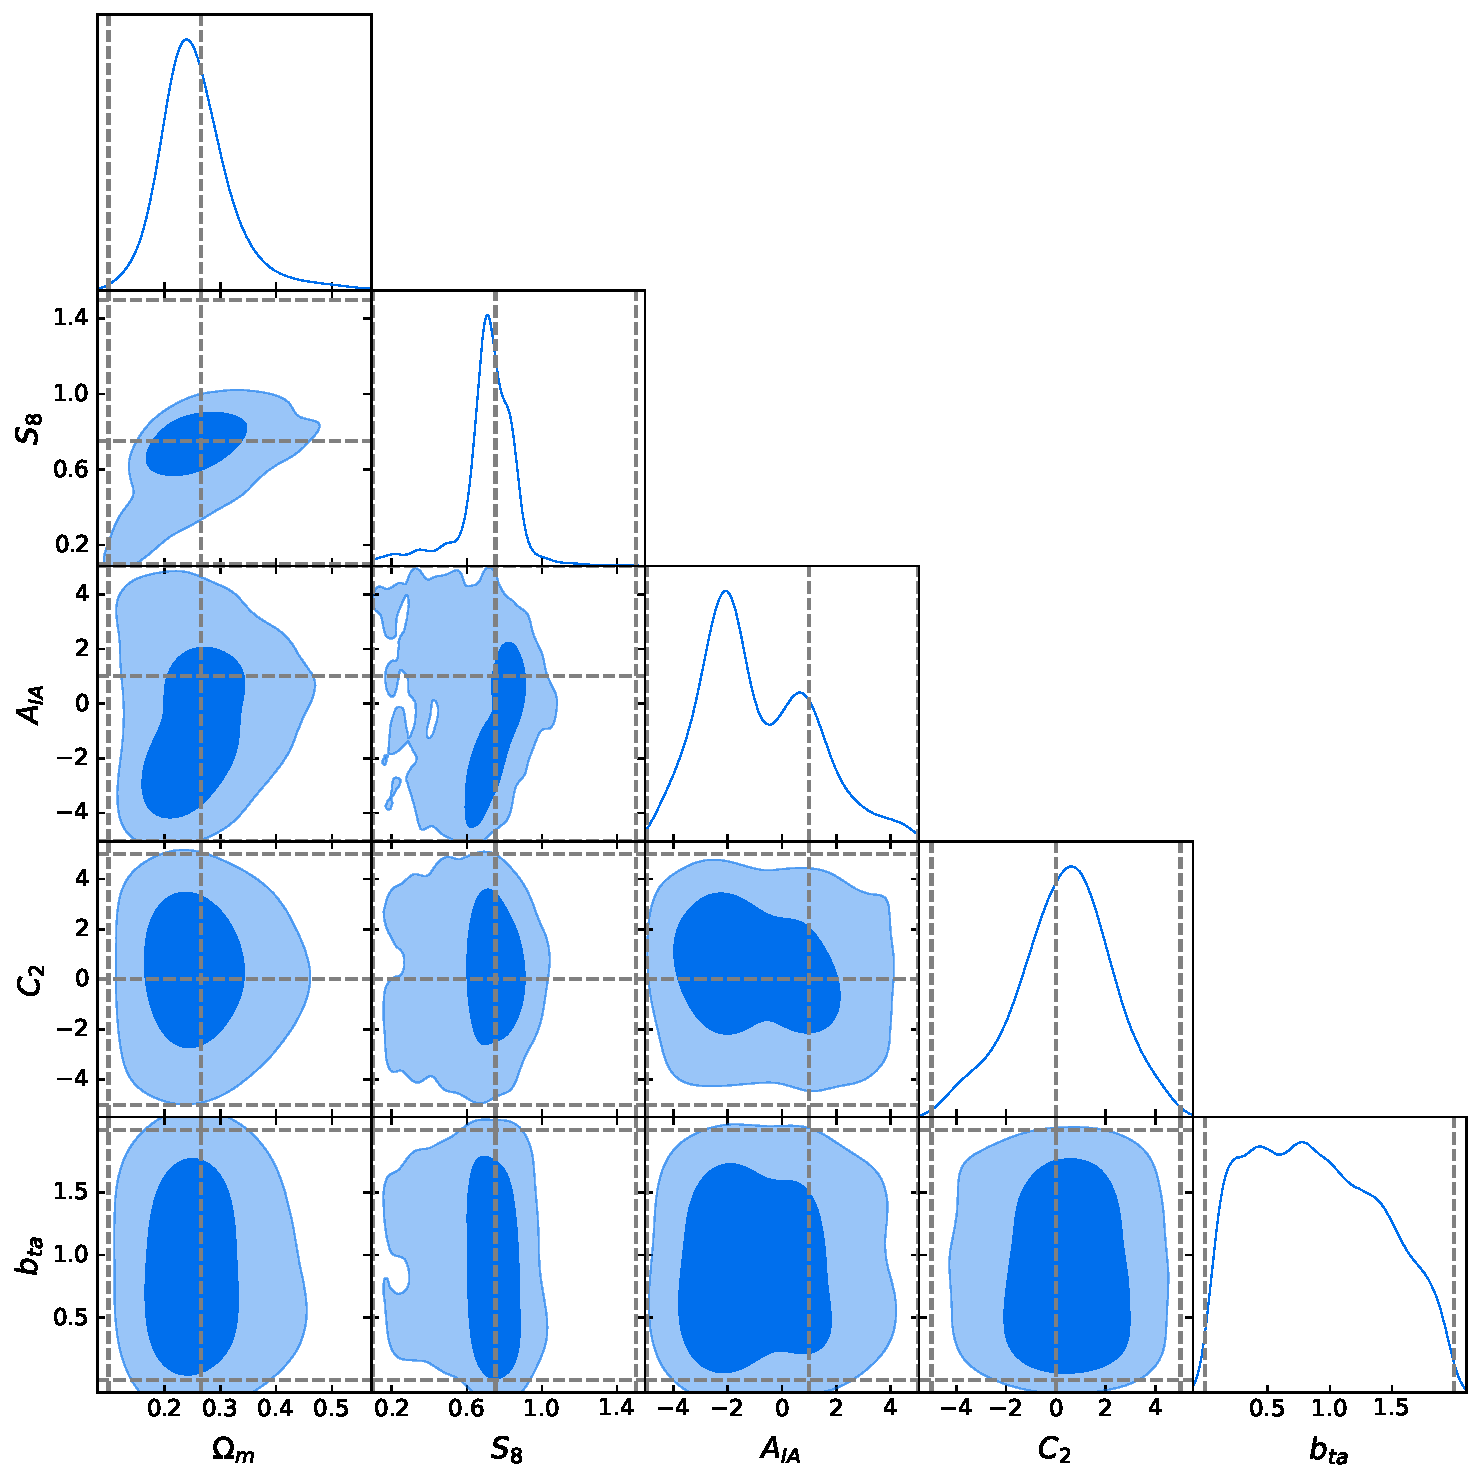
\includegraphics[width=\columnwidth]{graphs/triangle_nla_5D.pdf}
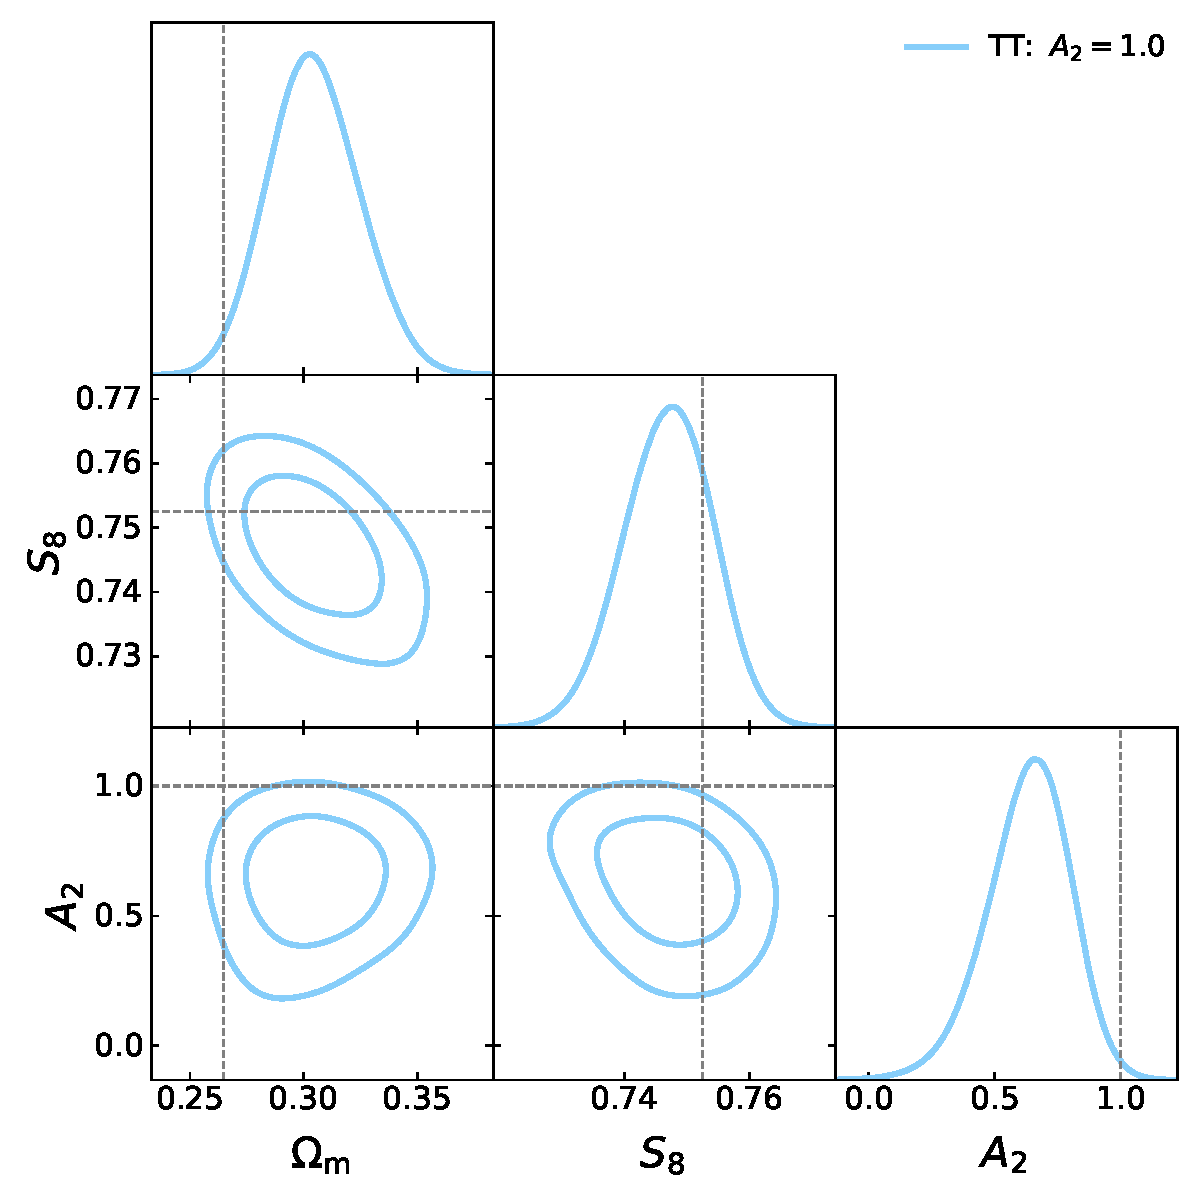
\includegraphics[width=\columnwidth]{graphs/TT_a2.pdf}
\caption{Cosmological inference from the TT-infused simulations, with $A_2$ varied ($A_1$ and $b_\mathrm{TA}$ fixed). The cross-hairs represent the truth as fixed in the {\it Outer Rim} $N$-body simulations \citep{OuterRim}.}
\label{fig:triangle_tt_vary_a2}
\end{figure}
